\chapter{Particle Production from Lepton-Nucleus Collisions}
\label{upc}

\section{Introduction}

Ever since Ernest Rutherford discovered the atomic nucleus by shining a beam of $\alpha$-particles onto a gold foil in the early twentieth century \cite{Rutherford:1911zz}, fixed target experiments have enjoyed a rich history of probing interatomic structure. With $\alpha$-particles used again by Rutherford in 1919 to discover the proton \cite{FRS:1919nrm} and by James Chadwick in 1932 to discover the neutron \cite{Chadwick:1932wcf}, a concrete theory of the atom was formed. The elements of the Periodic Table were forever stripped of their status as fundamental particles, replaced by the protons, neutrons, and electrons that comprise them.

This was not the end of the story. Showers of particles rained down from the heavens which did not fit neatly into this reductive description of the elements, and scattering experiments in the 1950s and `60s began producing these particles in experiments. Many of these particles were neatly described by Gell-Mann's Eightfold Way and quark model, which proposed that hadrons were built from more fundamental constituents. However, confirming the existence of such substructure in nucleons would require a beam of particles much smaller than the $\alpha$, which itself is a helium nucleus composed of two protons and two neutrons. Indeed, the first direct evidence for nucleon substructure came from the SLAC-MIT experiments of the late 1960s, which aimed high-energy electrons (notably {\it much} smaller than the $\alpha$) at fixed hydrogen and deuterium targets \cite{Bloom:1969kc,Breidenbach:1969kd}.  The resulting scattering distribution was consistent with the existence of three point-like constituents within the nucleons, providing the first direct evidence for quarks and lending strong support to the quark model. 


While fixed targets were originally used to probe the internal structure of nuclei and nucleons, SLAC repurposed some of their experimental infrastructure in the early 1980s to conduct searches for neutral particles produced in collisions between the beam and the target. At that time, theoretical interest had grown around the possible existence of light, long-lived particles, such as dark photons, right-handed neutrinos, and axions, whose weak coupling prevented direct-detection at other experiments. If one of the electrons in their fixed target experiments skirted by the nucleus of an atom in the target, it would still experience a coherent electromagnetic interaction with the nuclear Coulomb field, potentially receiving enough energy to go off-shell and produce one of these particles. The first experiment to search for such states was SLAC E137 \cite{Bjorken:1984mt}, and while the experiment concluded with null results, it inspired a new generation of {\it beam-dump} experiments\footnote{Conceptually, fixed target and beam dump experiments have similar collision set-ups, but the terms are used to distinguish the manner and scope of detection. Fixed target experiments typically have detectors much closer to the collision point, with the goal of capturing the incident beam particles to determine their deflection and hence the properties of the constituents within the target material. Beam dump experiments, on the other hand, typically have a detector far from the interaction point, with the goal of removing any SM background while allowing long-lived, neutral particles to propagate through empty space before decaying in or near the detector region.} like it. These include the electron beam-dump experiments E141 \cite{Riordan:1986wi}, E774 \cite{Bross:1989mp}, and NA64 \cite{Gninenko:2017acc}, the proton beam dump experiments CHARM \cite{CHARM:1985nku},  E613 \cite{Ball:1980ojt}, and NuCal \cite{Blumlein:2011mv}, and the ongoing muon beam dump experiment NA64$\mu$ \cite{Gertsenberger:2023ree}. 

None of these experiments has detected a new neutral particle, but they have refined the allowed parameter space of couplings and masses for these particles. Current bounds imply that if these particles exist, they are either {\it very} weakly interacting (with couplings $g \lesssim 10^{-8}$) or {\it not} very light (with masses $m \gtrsim 1~{\rm GeV}$), and perhaps a combination of both (for more detailed bounds, see e.g. \cite{Bauer:2021mvw,Batell:2022dpx}). Weaker couplings can be probed by increasing the luminosity of the beam dump or increasing the distance from the target to the detector, allowing long-lived particles to decay after passing through the shielding. Improving the mass reach is a different story, as it requires a substantial increase in the energy of the colliding beam. While this will be achieved at the Search for Hidden Particle (SHiP) with a $400~{\rm GeV}$ proton beam \cite{SHiP:2015vad, SHiP:2021nfo}, it is very difficult to accelerate electrons to hundreds of GeV or TeV of energy, in part due to their small mass. In particular, circular beams are typically required to accelerate particles to high energies, but the energy loss for a circular beam of particles with energy $E$ and mass $m$ goes as $P \propto (E/m)^4$.


A similar energy limitation was encountered in the deep-inelastic scattering experiments described before. After the discovery of the quark, nuclear substructure experiments focused on determining the parton distribution functions (PDFs) $f_i(x, Q^2)$, which characterize the probability that parton $i$ has momentum fraction $x$ when probed at a scale $Q^2$. The behavior of the PDFs at lower $x$ and higher $Q^2$ is crucial for accurate QCD predictions, but each of these requires high beam energy. A clear solution to this problem is to accelerate the ``fixed target'' as well, by colliding an electron beam with a similarly relativistic beam of nucleons or nuclei. The most notable experiment with this approach was the Hadron-Electron Ring Accelerator (HERA) experiment at DESY between 1992 and 2007, which collided $28~{\rm GeV}$ electrons with $920~{\rm GeV}$ protons, thereby probing the PDFs down to $x \sim 10^{-5}$ and up to $Q^2 \sim 10^5~{\rm GeV}^2$ \cite{Wichmann:2007zf}. More recently, the Electron-Ion Collider (EIC) is being constructed at Brookhaven National Lab (BNL) and is expected to begin operating by the early 2030s \cite{AbdulKhalek:2021gbh}. The EIC will collide $18~{\rm GeV}$ electrons with protons and heavy ions at up to $110~{\rm GeV}/{\rm nucleon}$. While the available energy is not as high at HERA, the luminosity is expected to be much larger, and the addition of heavy ion beams will allow for precise determination of PDFs for heavy nuclei down to $x \sim 10^{-4}$ and up to $Q^2 \sim 10^4~{\rm GeV}^2$ with high statistics. In particular, the electron in the frame of a heavy ion at the EIC will have $4~{\rm TeV}$ of energy, so the resulting cross-section has equivalent kinematics to a $4~{\rm TeV}$ electron beam dump experiment.

It is therefore worthwhile to investigate whether the EIC, and other lepton-nucleus collider experiments such as the Electron Ion Collider in China (EicC) \cite{Anderle:2021wcy}, would be able to probe the existence of neutral particles with heavier masses than the beam dump experiments before them. While these experiments lose out on luminosity relative to their predecessors (due to the lower density of the ion beam bunches as opposed to the high density target), their higher available energy may be advantageous for probing heavier neutral particles.


Of course, increasing collision energy is not limited to electron beams. Muons offer an attractive alternative, given that they lose much less energy than electrons from synchrotron radiation by a factor of $(m_e/m_\mu)^4 = 10^{-10}$. This fact has helped to fuel interest in the possibility of a multi-TeV muon collider in the future \cite{Delahaye:2013jla,Long:2020wfp,Accettura:2023ked}. As part of the research and development for such a collider, multi-TeV muon beam dumps will likely be produced, which could be incorporated into a high-energy muon beam dump experiment. In particular, Refs.~\cite{Cesarotti:2022ttv,Cesarotti:2023sje} have shown that muon beam dumps can probe muon-coupled neutral particles at mass scales well beyond those accessible to current or planned electron and proton experiments, extending the sensitivity well into the multi-GeV regime. A more ambitious possibility is the construction of a {\it muon-ion collider}. Such a facility could be realized as an upgrade to the EIC, or as an entirely new experiment built at a separate site. While the technical feasibility of a muon-ion collider is under investigation, there is evidence to suggest that it would be far-superior to a fixed-target experiment for nuclear physics applications \cite{Acosta:2021qpx,Acosta:2022ejc}, and it would excel at some BSM applications as well \cite{Davoudiasl:2024fiz}.

In this chapter, we will focus on characterizing the production mode $\ell A_Z \rightarrow \ell' A_Z \varphi$ at experiments which involve lepton-nucleus collisions, where $A_Z$ is a heavy ion and $\varphi$ is a neutral particle which can couple to the (pseudo)-scalar or (axial)-vector lepton currents. These results will be applied more directly to LFV ALPs in Chapter~\ref{alp_collider}, and hidden vector bosons in Chapter \ref{bosons}. For concreteness, we will apply our results to some of the existing, planned, and hypothetical detectors described above: 
\begin{enumerate}
    \item E137: E137 was a beam-dump experiment at SLAC which deposited a $20~{\rm GeV}$ electron beam into a block of Aluminum ($_{13}^{26}{\rm Al}$). While it did not make any new discoveries, its null results allow us to place limits on light, long-lived particles to this day. 
    \item EIC: The EIC is an upcoming experiment at BNL which will collide electrons with energies up to $18~{\rm GeV}$ and heavy ions with energies up to $110~{\rm GeV}$ per nucleon. While a variety of heavy ions will be used and the experiment will also operate in proton mode, here we will focus on the EIC in gold ($_{\ 79}^{197}{\rm Au}$) mode assuming an energy of $110~{\rm GeV}$/nucleon.
    \item MuBeD: ``MuBeD'' is our name for a hypothetical future (Mu)on (Be)am (D)ump experiment. We assume the muon beam has energy $1~{\rm TeV}$ and is incident on a block of lead ($_{\ 82}^{204}{\rm Pb}$). Given that we mainly discuss production cross-sections in this chapter, we defer specific assumptions about the surrounding detector apparatus to later chapters.
    \item MuSIC: The Muon (Synchrotron) Ion Collider is our name for a hypothetical upgrade to the EIC which replaces the electron beam with a 1 TeV muon beam. While the feasibility of such an upgrade is questionable, it provides a useful benchmark for comparison of lepton beam-dump experiments and lepton-ion colliders. For simplicity, we take the ion beam to be a $110~{\rm GeV}$ beam of Gold ($_{\ 79}^{197}{\rm Au}$) ions, in line with our benchmark EIC scenario.
\end{enumerate}
In Section \ref{sec:feasibility}, we discuss some conceptual aspects of the production process. In Section \ref{sec:form_factors}, we review our simplified model of atoms and their nuclei. In Section  \ref{sec:amplitude_calc},, we provide analytic expressions for the amplitudes and crosss-section, and compare the production cross-sections at each experiment. In Section \ref{sec:WW}, we compare the exact results to the Weizs\"acker-Williams approximation and Improved Weizs\"acker-Williams approximation. In Sections \ref{sec:phi_kin} and \ref{sec:l_kin}, we discuss the kinematic distributions of the final-state particles in the collision. Finally, in Section \ref{sec:lfv_scalar_case_study}, we apply the results of the chapter to examine limits on a scalar with an $e\tau$ or $\mu\tau$ flavor-violating interaction.


\section{Feasibility of Particle Production in Lepton-Nucleus Collisions}\label{sec:feasibility}
We will begin by discussing the kinematics of ultra-peripheral particle production in lepton-nucleus collisions. We are interested in the scenario in which the ion or nucleus acts as a source of photons for the incoming lepton. After a high-energy collision with one of these photons, a particle $\varphi$ is produced, potentially converting the lepton $\ell$ into a different lepton $\ell'$. Before moving to more technical results, it is worth considering just how massive the boson $\varphi$ can be. To do so, it is convenient to examine the collision in the rest-frame of the initial-state nucleus. Suppose in this frame, the lepton has energy $E$ and momentum ${\bf p}$, so that its four-momentum is
\beq
    p^\mu = \left(E, 0, 0, |{\bf p}|\right)
\eeq
with $E^2 = |{\bf p}|^2 + m_\ell^2$. Let $q^\mu = P_f^\mu- P_i^\mu$ be the four-momentum exchanged from the ion to the lepton, where $P_i^\mu$ and $P_f^\mu$ represent the initial and final-state four-momenta of the ion. The produced particle can be its heaviest when the smallest possible amount of momentum is imparted to the ion, so we assume the ion recoils along the beam axis. If this recoil momentum is $Q$, then
\begin{align}
    P_i^\mu = (M, 0, 0, 0), & & P_f^\mu = (\sqrt{M^2+Q^2}, 0, 0, Q).
\end{align}
As long as the recoil momentum of the nucleus is small relative to its mass,  we have 
\begin{align}
    q^\mu \approx \left(\frac{Q^2}{2M}, 0, 0, -Q\right).
\end{align}
Finally, let the combined four-momentum of the final-state lepton $\ell'$ and boson $\varphi$ be $p_{\varphi \ell'}^\mu$. Then, conservation of four-momentum implies
\begin{align}
    p^\mu - q^\mu = p_{\varphi\ell'}^\mu
\end{align}
As a consequence of the Cauchy-Schwartz inequality, $p_{\varphi\ell'}^2 \geq (m_\varphi + m_{\ell'})^2$. Also, under the assumption that $E, |{\bf p}_\ell|\gg m_\ell$, we have $(p - q)^2 \approx 2Q|{\bf p}|$. We can use this to place a limit on the mass $m_\varphi$ of the boson:
\begin{align}
    (p - q)^2 \approx 2Q|{\bf p}| = p_{\varphi \ell'}^2   &\geq (m_\varphi + m_{\ell'})^2\\
    \implies m_\varphi + m_{\ell'} \leq \sqrt{2Q|{\bf p}|}.
\end{align}
Therefore, the mass of the produced  boson is limited by $m_\varphi + m_{\ell'} \leq \sqrt{2Q|{\bf p}|}$, where $Q$ is the transfer-momentum of the exchanged photon and $|{\bf p}|$ is the initial-state lepton momentum in the rest frame of the initial-state ion. 

If one limits the analysis to coherent interaction of the lepton with the nucleus, this limits the photon transfer momentum to to $Q \lesssim 1/r_{A} \sim 100\,{\rm MeV}$,\footnote{Technically, the coherent nuclear form-factor is still non-zero at higher values of $Q$, but it is very small, so the cross-section of producing heavier particles coherently is severely suppressed.} where $r_A$ is the radius of the ion. For the benchmark experiments considered in the introduction, this corresponds to $m_\varphi \lesssim 2\,{\rm GeV}$ at E137, $m_\varphi \lesssim {30\rm GeV}$ at the EIC, $m_\varphi \lesssim 15~{\rm GeV}$ at MuBeD, and $m_\varphi \lesssim 60~{\rm GeV}$ at MuSIC. Alternatively, if one is willing to sacrifice coherence and interact electromagnetically with the protons within the nucleus, it is possible to push $Q$ to $1/r_p \sim 1\,{\rm GeV}$, where $r_p$ is the proton radius. In this case, $m_\varphi \lesssim 6~{\rm GeV}$ at E137, $m_\varphi \lesssim 90~{\rm GeV}$ at the EIC, $m_\varphi \lesssim 45~{\rm GeV}$ at MuBeD, and $m_\varphi \lesssim 200~{\rm GeV}$ at MuSIC. In principle, it is possible to push beyond this and consider deep inelastic scattering within the nucleons, but the cross-sections for this process will be severely suppressed.

\section{Nuclear and Atomic Form-Factors}\label{sec:form_factors}
In order to compute the cross-section for peripheral production of a boson, we must know how the lepton interacts electromagnetically with the nucleus. This is encoded with the electromagnetic nuclear and atomic form-factors. In general, the electromagnetic form-factor of the nucleus receives a coherent contribution from the nucleus as a whole and an incoherent contribution from the individual protons and neutrons within the nucleus.\footnote{There is also the possibility of deep-inelastic scattering with the quarks within the nucleons, but we do not consider that here.} For the coherent nuclear form-factor, we use an approximation of the Fourier transform of the Woods-Saxon distribution ~\cite{Klein:1999qj}, given by
\begin{align}
    G_{\rm coh}^{\rm nuc}(t) &= \frac{9Z^2}{(R_A\sqrt{t})^6}\left[\left(\sin{(R_A\sqrt{t})} - R_A \sqrt{t}\cos{(R_A\sqrt{t})}\right)\frac{1}{1+a_0^2t}\right]^2\label{eq:nuc_ff_coh}
\end{align}
where $a_0 = 0.79\,{\rm fm}$ and $R_A = (1.2\,{\rm fm})A^{1/3}$. Note that for small $t$, this agrees with the form of the coherent nuclear form-factor used in Refs.~\cite{Kim:1973he,Tsai:1973py}, but falls off more quickly at larger $t$ ($\sim 1/t^5$ instead of $\sim 1/t^2$). 
For the incoherent nuclear form factor, we use the dipole approximation for the electromagnetic form-factors of the nucleons within the nucleus~\cite{Kim:1973he,Tsai:1973py},
\begin{align}
    G_{\rm incoh}^{\rm nuc}(t) &= \frac{1}{(1+t/t_0)^4(1+t/4m_p^2)}\left[Z(1+(\mu_p^2/4m_p^2)t + (A-Z)(\mu_n^2/4m_p^2)t\right]
\end{align}
The dipole approximation becomes less accurate at higher momentum transfer \cite{Qattan:2024pco}, so to be safe, we impose a cut-off on the form-factors at $t = 1~{\rm GeV}$.

In the case that the nucleus is inside of an atom (as opposed to being a stripped ion), one must also parametrize shielding from the electron shells. This is accomplished with the atomic form-factors. Following Refs.~\cite{Kim:1973he,Tsai:1973py}, we take the coherent and incoherent atomic form-factors to be 
\begin{align}
    G_{\rm coh}^{\rm atom}(t) = \left[\frac{a^2t}{1+a^2t}\right]^2, && G_{\rm incoh}^{\rm atom}(t) = \left[\frac{a'^2t}{1+a'^2t}\right]^2
\end{align}
with $a = 111Z^{-1/3}/m_e$ and $a' = 571.4Z^{-2/3}/m_e$. 

Throughout this chapter and subsequent chapters, we will only focus on {\it coherent} production of particles at the EIC and MuSIC, as this will allow us to avoid potentially high background from breakup of the nucleus. For the beam-dump experiments, on the other hand, we will consider the full coherent and incoherent nuclear and atomic form-factors.

\section{Amplitude Calculation}\label{sec:amplitude_calc}
Now we will compute the amplitude for peripheral particle production in lepton-nucleus collisions. 
This process is often treated with the Weizs\"acker-Williams approximation, but this can potentially over-estimate the differential cross-section in some regions of the parameter space. Hence, we opt to evaluate the tree-level diagram exactly; we will compare the exact results to the Weizs\"acker-Williams approximation in Section \ref{sec:WW}. A similar analysis was performed in Refs.~\cite{Liu:2016mqv,Liu:2017htz}, but we treat the situation more generally, allowing for CLFV interactions and arbitrary PV. While we restrict our analysis to CLFV processes, we note that the initial and final-state charged leptons can be replaced with any fermion in this analysis without any qualitative differences.

\begin{figure}
    \centering
    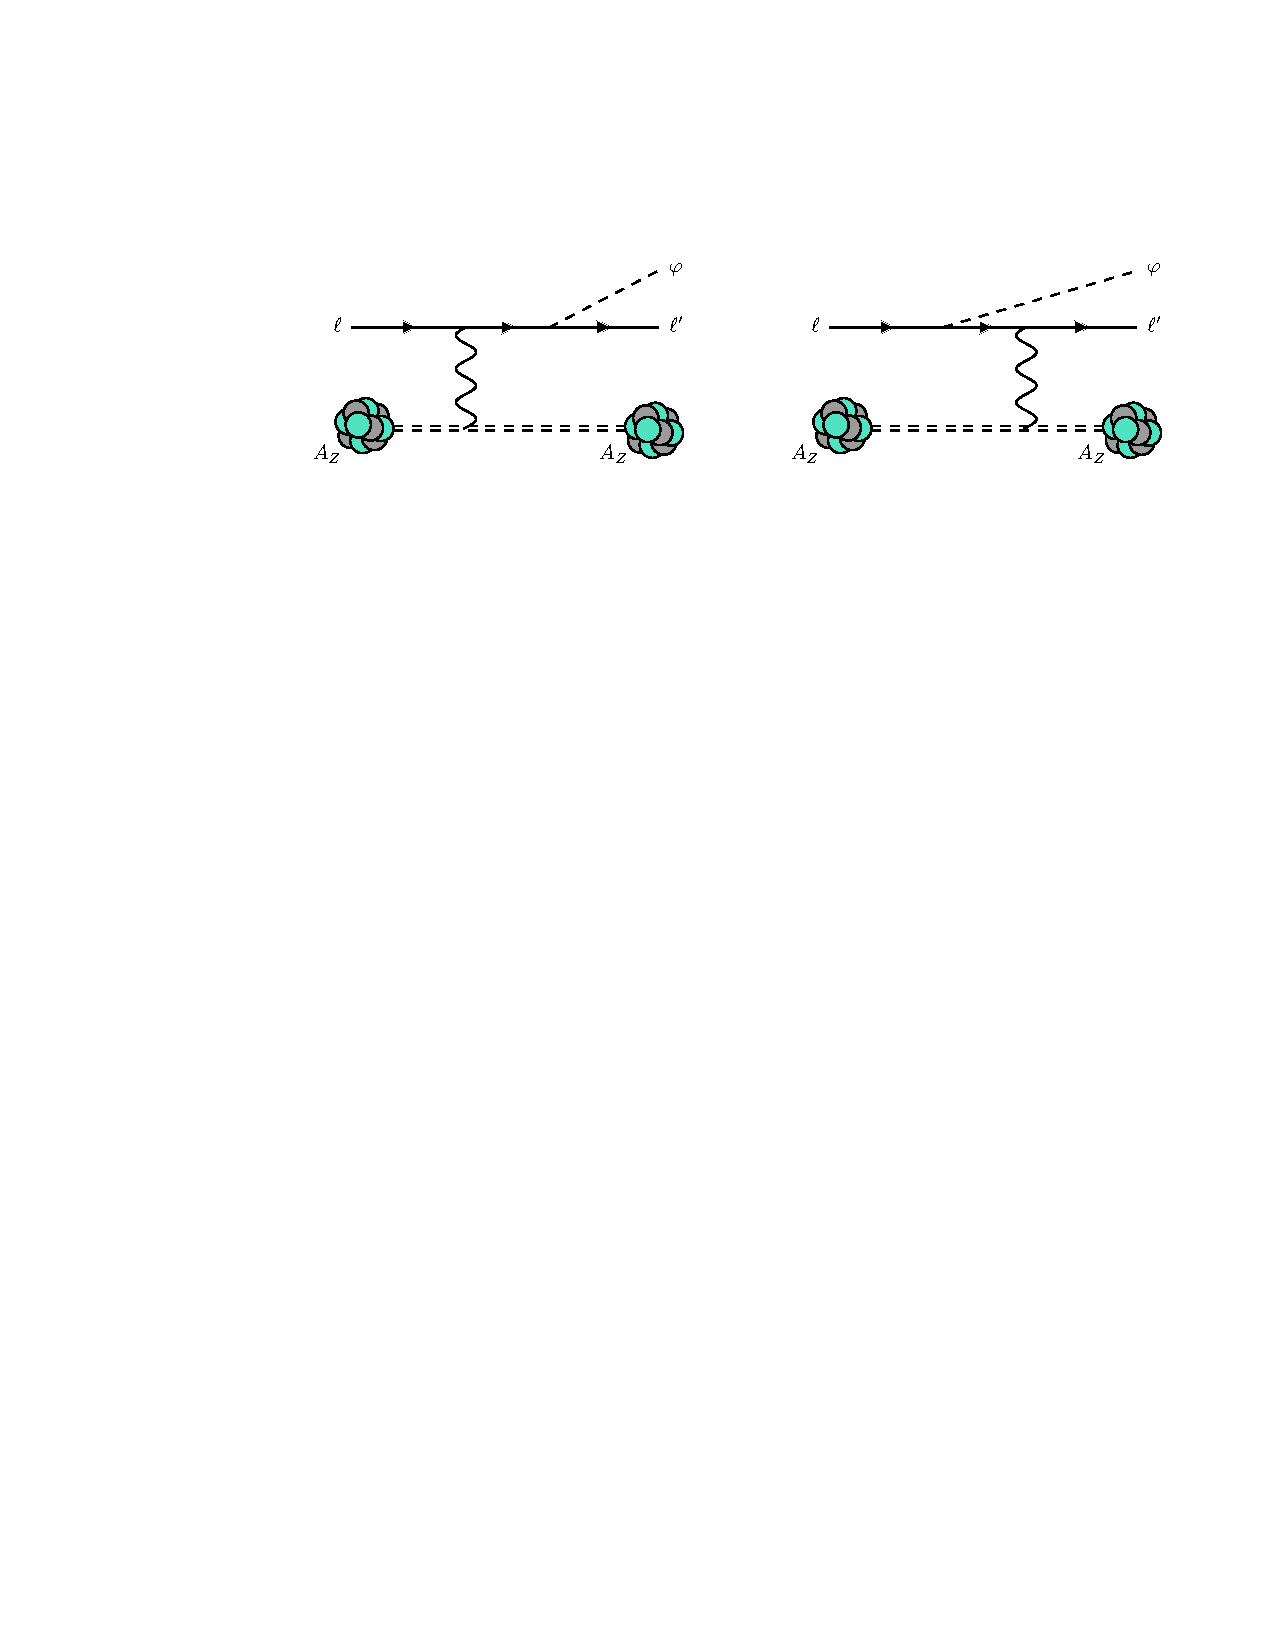
\includegraphics[width=\linewidth]{figures/chapter4/production_diagram.pdf}
    \caption{Relevant Feynman diagrams for the process $\ell A_Z \rightarrow \ell' A_Z \varphi$ via photon exchange.} 
    \label{fig:production_diagram}
\end{figure}

The diagrams relevant for this process are shown in Fig.~\ref{fig:production_diagram}. We take $p^\mu = (E, {\bf p})$ to be four-momentum of the initial state lepton, $P_i^\mu$ and $P_f^\mu$ to be the four-momenta of the initial and final-state nucleus, $p'^\mu = (E', {\bf p}')$ to be the four-momentum of the final-state $\ell'$, and $k^\mu = (E_k, {\bf k})$ to be the four-momentum of the final-state $\varphi$. It is additionally useful to define the transfer momentum $q^\mu = P_f^\mu - P_i^\mu$ and the sum $P^\mu = P_f^\mu + P_i^\mu$, along with the Mandelstam variables
\begin{align}
    s &= (p'+k)^2 - m_\ell^2 = 2p'\cdot k + m_\varphi^2 + m_{\ell'}^2 - m_\ell^2 \\
    u &= (p-k)^2 - m_{\ell'}^2 = -2p\cdot k + m_\varphi^2 + m_\ell^2  - m_{\ell'}^2\\
    t_2 &= (p' - p)^2 = -2p'\cdot p + m_\ell^2 + m_{\ell'}^2 \\
    t &= -q^2.
\end{align}
The lepton-photon vertex is the standard QED vertex. The photon-ion vertex is parametrized by a form-factor $F(q^2)$, so that 
\begin{equation}
    V^\mu_{A_Z\gamma} = ieF(q^2) P^\mu
\end{equation}
where the details of the form-factor were discussed in Section \ref{sec:form_factors}. For stripped ions, $F(q^2 \rightarrow 0) = Z$, where $Ze$ is the charge of the nucleus. In this low-$q^2$ regime, the incoming lepton views the nucleus as a whole as a coherent source of photons. For nuclei that are within atoms in materials (such as in fixed-target or beam-dump experiments) $F(q^2\rightarrow 0) = 0$, as the charge of the nuclei is shielded by the electron shell at large distances. However, there is still a coherent regime $1/r_{A_Z}^2 > q^2 > Z^2/r_{\rm Bohr}^2$ for which $F(q^2) \approx Z$. The only other vertex is the $\varphi$-$\ell$-$\ell'$ vertex. We consider  scalars with interaction vertex
\beq
    V_{\varphi \ell \ell'} = ige^{i\phi}(\cos{\theta}+\gamma_5e^{i\delta}\sin{\theta})\label{eq:scalar_vertex}
\eeq
and vectors with interaction vertex
\beq
    V_{\varphi \ell \ell'}^\mu = ige^{i\phi}\gamma^\mu(\cos{\theta}+\gamma_5e^{i\delta}\sin{\theta}).\label{eq:vector_vertex}
\eeq
Following the discussions in Chapters 2 and 3, we note that the scalar interaction in Eq.~\ref{eq:scalar_vertex} can easily be recast to apply to ALPs. The amplitude for the process in Feynman gauge is then given by
\begin{equation}
    i{\cal M} = \left[F(q^2)P^\mu\right]\frac{ige^2}{q^2}e^{i\phi}\left[\bar{u}(p')\Gamma_\mu(p, p', k)u(p)\right]
\end{equation}
with 
\begin{equation}
    \Gamma_\mu^S =  \gamma_\mu \frac{1}{\slashed{p}-\slashed{k}-m_{\ell'}}(\cos{\theta}+\gamma_5 e^{i\delta}\sin{\theta})+(\cos{\theta}+\gamma_5 e^{i\delta}\sin{\theta})\frac{1}{\slashed{p}'+\slashed{k}-m_\ell}\gamma_\mu \label{eq:scalar_vertex}
\end{equation}
for scalars and
\begin{equation}
    \Gamma_\mu^V =  \epsilon^\alpha(k)\left[\gamma_\mu \frac{1}{\slashed{p}-\slashed{k}-m_{\ell'}}\gamma_\alpha(\cos{\theta}+\gamma_5 e^{i\delta}\sin{\theta})+\gamma_\alpha(\cos{\theta}+\gamma_5 e^{i\delta}\sin{\theta})\frac{1}{\slashed{p}'+\slashed{k}-m_\ell}\gamma_\mu\right]\label{eq:vector_vertex}
\end{equation}
for vectors.
We are now equipped to compute the differential cross-section for producing a scalar and vector via lepton-nucleus collisions. The spin-averaged squared amplitude is given by
\begin{equation}
    \overline{|{\cal M}|^2} = g^2 e^4 \frac{F(q^2)^2}{q^2}\overline{|{\cal A}|^2}
\end{equation}
where in general, the amplitude can be decomposed as $\overline{|{\cal A}|^2} = \overline{|{\cal A}_0|^2} + \overline{|{\cal A}_{\rm PV}|^2}\sin^2{\theta}$. The label ``PV'' refers to the fact that the angle $\theta$, absent the other couplings, controls the degree of PV in the interaction. At tree-level, the phases $\phi$ and $\delta$ drop out of the calculation. The amplitudes for the scalar scenario are given by
\begin{align}
    \overline{|{\cal A}_{S,0}|^2} &=  \frac{(s+u)^2}{su}P^2 - 4\frac{t}{su}(P\cdot k)^2\nonumber \\
    &\ \ \ + \frac{(s+u)^2}{s^2u^2}\left(m_\varphi^2 - (m_{\ell} + m_{\ell'})^2\right)\left[P^2t - 4\left(\frac{uP\cdot p + sP\cdot p'}{s+u}\right)^2\right]\,\nonumber\\
    \overline{|{\cal A}_{S,{\rm PV}}|^2} &= 4m_{\ell}m_{\ell'}\frac{(s+u)^2}{s^2u^2}\left[P^2t - 4\left(\frac{uP\cdot p + sP\cdot p'}{s+u}\right)^2\right]\,.\label{eq:scalar_amplitudes}
\end{align}
And for the vector scenario (using $\Delta m_{\ell\ell'}^2 = (m_{\ell'} - m_\ell)^2$)), 
\begin{align}
    \overline{|{\cal A}_{V,0}|^2} &= \left[\frac{(s+u)^2}{su}\left(2+\frac{\Delta m_{\ell\ell'}^2}{m_\varphi^2}\right) - 4\right]P^2 - 4\frac{t}{su}\frac{\Delta m_{\ell\ell'}^2}{m_\varphi^2}(P\cdot k)^2\nonumber\\
    &\ \ \ \ - 8\frac{t}{su}\left[(P\cdot p)^2 + (P\cdot p')^2 +\frac{t_2+m_{\varphi}^2-2\Delta m_{\ell\ell'}^2}{2}P^2\right]\nonumber \\ & \ \ \ \ + \frac{(s+u)^2}{s^2u^2}\left(1 - \frac{\Delta m_{\ell\ell'}^2}{m_\varphi^2}\right)\left(2m_{\varphi}^2 + (m_\ell + m_{\ell'})^2\right)\left[P^2t - 4\left(\frac{uP\cdot p + sP\cdot p'}{s+u}\right)^2\right] \nonumber\\
    \overline{|{\cal A}_{V,{\rm PV}}|^2} &= \frac{4m_{\ell}m_{\ell'}}{m_{\varphi}^2}\left[\frac{(s+u)^2}{su} P^2 - 4\frac{t}{su}(P\cdot k)^2 + 8m_{\varphi}^2\frac{t}{su}P^2\right.\nonumber\\
    &\ \ \ \ \ \ \ \ \left. - 3m_{\varphi}^2\frac{(s+u)^2}{s^2u^2}\left[P^2t - 4\left(\frac{uP\cdot p + sP\cdot p'}{s+u}\right)^2\right]\right].\label{eq:vector_amplitudes}
\end{align}
These results are in agreement with Refs.~\cite{Liu:2016mqv,Liu:2017htz} for the special case $\ell' = \ell$ and $\theta = 0$, $\pi/2$.\footnote{The apparent sign disagreements with these references are due to a difference in metric convention.} Here, we note that the PV contributions to each amplitude are suppressed both for $m_\ell \neq m_{\ell'}$ (due to the lepton mass hierarchy) and $m_\ell,m_{\ell'} \ll m_\varphi$. However, PV effects can become significant for $m_\varphi \ll m_\ell = m_{\ell'}$, especially for light on-diagonal vectors, for which the PV contributions are proportional to $4m_\ell^2/m_\varphi^2$. This effect could be utilized to provide more stringent constraints on PV vectors compared to their PC counterparts.

\subsection{Phase-Space Integration}
We perform the cross-section integration in the rest-frame of the ion. The differential cross-section is given by
\begin{align}
    d\sigma &= \frac{1}{(2E)(2M)|{\bf v}|}|{\cal M}|^2 (2\pi)^4 \delta^{(4)}(p' + k - p - q)\frac{d^3 p'}{(2\pi)^3 2E'}\frac{d^3 P_f}{(2\pi)^3 2E_f}\frac{d^3 k}{(2\pi)^3 2E_k}
\end{align}
where ${\bf v}$ is the velocity of the incoming electron, so $|{\bf v}| = |{\bf p}|/E$. Using this and simplifying the denominators yields
\begin{align}
    d\sigma &= \frac{1}{1024 \pi^5 |{\bf p}| M E'E_f E_k}|{\cal M}|^2\delta^{(4)}(p' + k - p - q) d^3 {\bf p}' d^3 {\bf P}_f d^3{\bf k}.
\end{align}
It is then possible to split the four-momentum-conserving $\delta$-function into energy- conserving and momentum-conserving $\delta$ functions, then integrate over $p'$ to remove the momentum-conserving $\delta$-function. Also trading $P_f$ with $q = P_f - P_i$, we have  
\begin{align}
    d\sigma &= \frac{1}{1024 \pi^5 |{\bf p}| M E'E_f E_k}|{\cal M}|^2\delta(E' + E_k - E - q_0) d^3 {\bf q}\,d^3{\bf k}.
\end{align}
At this point, it is useful to define ${\bf V} = {\bf p} - {\bf k}$ with $V = |{\bf V}|$, and then decompose ${\bf q}=(Q, \theta_q, \phi_q)$ in spherical coordinates with $z$-axis pointed along ${\bf V}$. Then, one can show
\begin{equation}
    \delta(E' + E_k - E - q_0) = \frac{E'}{QV}\delta(\cos{\theta_q} - \cos{\theta_q^0})
\end{equation}
where 
\begin{equation}
\cos{\theta_q^0} = \frac{u - \left(1+\frac{E-E_k}{M}\right)t}{2QV}.
\end{equation}
As a result, the integral over $\cos{\theta_q}$ can be performed, collapsing the $\delta$-function. Decomposing ${\bf k} = (|{\bf k}|, \cos{\theta_k}, \phi_k)$ in spherical coordinates with $z$-axis along the beam axis, the integrand is independent of $\phi_k$, so this can be integrated over as well. The resulting differential cross-section is 
\begin{align}
    d\sigma = \frac{1}{1024\pi^5|{\bf p}|ME_f E_k QV}|{\cal M}|^2\Theta(1 - \cos^2{\theta_q^0})Q^2 dQ\,d\phi_q\,|{\bf k}|^2 d|{\bf k}|d(\cos{\theta_k}).
\end{align}
Now, we can replace the integral over $Q$ with an integral over the Mandelstam variable $t$ via the substitution $dQ = E_f dt/(2MQ)$, and we can replace the integral over $|{\bf k}|$ with an integral over the energy of the $\varphi$ particle $E_k$. This gives us the energy-angle differential cross-section
\begin{align}
    \frac{d\sigma}{dE_k\,d\theta_k} &= \frac{\sin{\theta_k}}{64\pi^3}\frac{|{\bf k}|}{|{\bf p}|V}\int_{t_-}^{t_+}dt\left(\frac{1}{8M^2}\int_0^{2\pi}\frac{d\phi_q}{2\pi}|{\cal M}|^2\right).\label{eq:dsig}
\end{align}
Here, $t_{\pm}$ are the solutions to $\cos^2{\theta_{q}^0} = 1$. They are given by
\begin{align}
    t_+ &= \frac{M\left[(E-E_k+M)u + 2MV^2 + V\sqrt{4M^2V^2+[4M(E-E_k+M) + u]u}\right]}{(E-E_k+M)^2 - V^2} \label{eq:t_+}\\
    t_- &= \frac{Mu^2}{(E-E_k+M)u + 2MV^2 + V\sqrt{4M^2V^2+[4M(E-E_k+M) + u]u}}.\label{eq:t_-}
\end{align}
Rather than rationalizing the denominator in $t_-$, we find it convenient to keep the present form for numerical evaluation, as this avoids large cancellations which result in floating-point errors. Alternatively, one can integrate over a wider range of $t$ and keep the Heaviside function $\Theta(1-\cos^2{\theta_q^0})$ in the integrand.

As it turns out, the angular integral in Eq.~\ref{eq:dsig} is exactly solvable for the amplitudes in Eqs.~\ref{eq:scalar_amplitudes} and \ref{eq:vector_amplitudes}. All of the dependence on $\phi_q$ enters through the dot-product
\begin{align}
    {\bf q}\cdot{\bf p} &= \frac{Q|{\bf p}|}{V}\left[|{\bf p}|\cos{\theta_q^0} - |{\bf k}|(\cos{\theta_q^0}\cos{\theta_k} - \sin{\theta_q^0}\sin{\theta_k}\cos{\phi_q})\right],
\end{align}
which in turn appears in $s$. In particular, the necessary substitutions in terms of the integration variables are
\begin{align}
    s &= -\left(1+\frac{E}{M}\right)t + 2({\bf q}\cdot{\bf p}) \label{eq:s}\\
    u &= (E-E_k)^2 - V^2 - m_f^2\\ 
    t_2 &= m_\varphi^2 - s - u - t\\
    P^2 &= 4M^2 + t\\
    P\cdot p &= 2ME - \frac{1}{2}(s+t)\\
    P\cdot k &= 4ME_k - \frac{1}{2}(s+u)\\
    P\cdot p'&= 2M(E - E_k) + \frac{1}{2}(u-t).
\end{align}
Examining the amplitudes, we see that $\phi_q$ appears only as $\cos{\phi_q}$, which only appears in the denominator within powers of $s$ up to $s^2$. Then, each term can be written as
\begin{align}
    {\cal F}_k(\{{\cal Q}_i\}, s) = \frac{{\cal Q}_0 + {\cal Q}_1 s + {\cal Q}_2 s^2}{s^k}
\end{align}
with $k = 0$ or $1$. The integral over these terms is straightforward using methods from complex analysis. Hence, the $E_k$-$\theta_k$ differential cross-section can be computed with a single integral over the photon transfer $t$. 

\subsection{Features of the Production Cross-Section}

In this section, we present results for the total production cross-section $\sigma(\ell A_Z\rightarrow \ell'A_Z\varphi)$. We choose a hard maximum cut-off on the transfer momentum of $t_+ = 1/r_p = 1~{\rm GeV}$. Beyond this point, there is still a contribution to the cross-section from deep-inelastic scattering off the quarks inside the nucleons, but the cross-section would be far too small to measure in the contexts we are considering. Given the generality of the discussion above, there are many parameters to consider; namely the details of the experiment (beam energy, nucleus species, and initial-state lepton) and the details of the interaction (vector or scalar-like interaction current, degree of PV in the coupling, and final-state lepton). We explore the effect of all of these parameters in Fig.~\ref{fig:production_crossx}, which plots the production cross-section of the particle $\varphi$ as a function of its mass $m_\varphi$. In particular, the top panels represent production of the $\varphi$ at experiments involving an electron beam (E137 and EIC), while the bottom panels represent production of  the $\varphi$ at hypothetical experiments involving a muon beam (MuBeD and MuSIC, described in the introduction). The panels on the left represent production of a (pseudo)scalar $\varphi$, whereas the panels on the right represent production of an (axial) vector $\varphi$. To account for all PV couplings, we note that the cross-section can always be written as $\sigma(\theta) = \sigma_0 + \sigma_{PV}\sin^2{\theta}$, where $\theta$ is an angle characterizing the degree of PV in the coupling. Hence, we shade between $\sigma(0)$ and $\sigma(\pi/2)$, although this is only noticeable in some of the plots in the lower panel. Finally, within each panel, the cross-section for production of a $\varphi$ and an $e$ (solid), $\mu$ (dashed) and $\tau$ (dotted) is shown. We note that while these plots represent the {\it production} cross-section of the particle $\varphi$ at each of these experiments, the actual signal cross-section is often much smaller, due in part to signal selection but mostly to detector efficiency and geometry. We will explore this in the context of the $\varphi$'s lab-frame kinematic distributions in Section \ref{sec:phi_kin}.
\begin{figure}[t!]
    \centering
    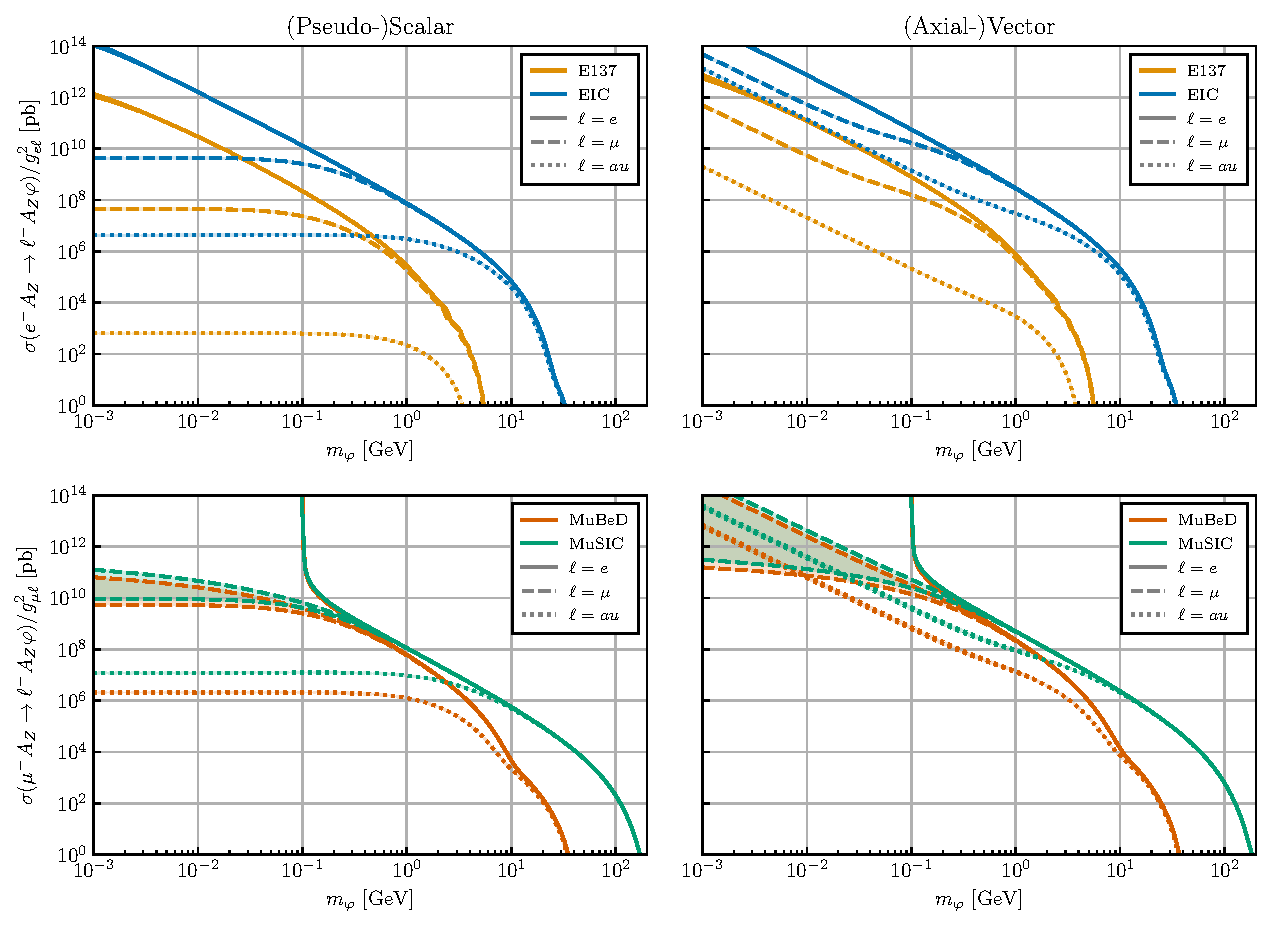
\includegraphics[trim={1cm 0 0.5cm 0}, width=\linewidth]{figures/chapter4/production_crossx.pdf}
    \caption[Production cross-sections for the process $\ell A_Z \rightarrow \ell' A_Z\varphi$ at various lepton-nucleus collision experiments.]{{\it Production} cross-sections for the processes ($\ell A_Z \rightarrow \ell' A_Z\varphi$ for $\ell' = e,\mu,\tau$), particle-types (scalar (left) and vector (right)), and lepton collision experiments (E137, EIC (top) and MuBeD, MuSIC (bottom)) discussed in the text. To account for PV couplings, we note that the production cross-section can always be written as $\sigma(\theta) = \sigma_0 + \sin^2{(\theta)}\sigma_{PV}$, so we shade the area between $\sigma(0)$ and $\sigma(\pi/2)$. PV effects only appear important for flavor-conserving production modes at the muon-nucleus colliders (dashed, bottom) when $m_\varphi < m_\mu$, although we expect that there is also a substantial difference at electron-nucleus colliders when $m_\varphi < m_e$.}
    \label{fig:production_crossx}
\end{figure}

We begin by examining the light $m_\varphi$ regime in Fig.~\ref{fig:production_crossx}. For light masses, the difference between lepton beam-dumps and lepton-ion collisions is largely insubstantial. In the electron case, we see that the cross-sections are larger for the EIC than E137, but this is mostly due to the difference in the charge of the nucleus involved with the collision (aluminum with $Z = 13$ for E137 and gold with $Z = 79$ for the EIC), as well as the additional available energy at the EIC in the rest frame of the gold ion. The comparison between lepton beam-dumps and lepton ion-collisions is more straightforward for the hypothetical muon collision experiments we consider, which have the same lepton beam energy ($E = 1~{\rm TeV}$) and nucleus charge (lead with $Z = 82$). In this case, we see in the bottom of Fig.~\ref{fig:production_crossx} that there is only a minor increase in the production cross-section for light $m_\varphi$ at MuSIC compared to at MuBeD. Coupled with the fact that beam-dump experiments will most definitely have a higher luminosity and favorable detector geometry for forward-produced particles, it appears that they are preferable over lepton-ion colliders for probing the existence of light particles. 

While one may take this to be a statement about the inefficacy of lepton-ion colliders for probing lighter-mass particles, it can be understood as a more general statement about the diminishing returns of higher-energy beams. To understand this, we note that in the rest-frame of the ion, the electron beam at the EIC will have an energy $E \approx 4~{\rm TeV}$, as opposed to E137's energy of $E = 20~{\rm GeV}$, and the muon beam at MuSIC would have a whopping $E \approx 20~{\rm TeV}$ of energy as opposed to MuBeD's $E = 1~{\rm TeV}$ of energy. Despite these large differences in energy, there is not much of an increase in the production cross-section.

Whereas lepton-ion collisions may not have much to offer in terms of probing lighter-mass particles, they have a much larger mass reach than their beam-dump counterparts. This is unsurprising given the additional available energy in the collisions, and highlights the main advantage of lepton-ion colliders, at least as far as peripheral particle production is concerned. In particular, with the hard cut-off of $t_+ = 1~{\rm GeV}$, the maximum producible particle via this process at the EIC and MuSIC are $m_\varphi = 95~{\rm GeV}$ and $200~{\rm GeV}$ respectively, as opposed to $m_\varphi = 6~{\rm GeV}$ and $44~{\rm GeV}$ at E137 and MuBeD respectively. 

Apart from the discrepancies between lepton beam dumps and lepton-ion colliders, we can also glean some insight into how PV in the interaction affect the cross-section. As anticipated in the end of Section \ref{sec:amplitude_calc}, PV effects are only significant for $m_\varphi < m_\ell = m_{\ell'}$. Given that the lower-bound on the plots is $m_\varphi = 1~{\rm MeV} > m_e$, these effects are only noticeable in the bottom plots. PV effects are especially dramatic in the vector scenario, for which there is a factor of $\sim 10^2$ increase in the cross-section for axial-vectors as opposed to pure vectors at $m_\varphi = 10~{\rm MeV}$.

In context of the results from Chapter \ref{lfv}, the PV-independence of the cross-sections for large $m_\varphi$ is notable. In particular, it was found in Section \ref{sec:lfv_limits} that limits on scalar LFV couplings $g_{\ell\ell'}$ can be substantially weaker for chiral scalars than pure scalars. In contrast, limits placed on the LFV couplings at lepton-nucleus collision experiments are largely immune to the PV details of the interaction, especially for large $m_\varphi$. At the same time, lepton-nucleus colliders with polarization-control such as the EIC will still have the ability to distinguish between PC and PV interactions in the event that such a particle is found. To see this, we note that the interaction between a scalar $\varphi$, $\ell$, and $\ell'$ can be rewritten
\begin{align}
    {\cal L}_{\varphi \ell \ell'} = g_{\ell \ell'}e^{i\phi} \left[(\cos{\theta} - ie^{i\delta} \sin{\theta})\varphi\bar{\ell}'P_L\ell + (\cos{\theta} + ie^{i\delta} \sin{\theta})\varphi\bar{\ell}'P_R\ell\right] + {\rm H.c.}
\end{align}
The left- and right-polarized cross-sections can be found by isolating each of these terms. Using $\sigma(\theta) = \sigma_0 + \sigma_{PV}\sin^2{\theta}$ to represent the unpolarized cross-section, we see that we can set $\theta = \pi/4$ ($-\pi/4$) to isolate $\sigma_R$ ($\sigma_L$), provided we modify the coupling to account for the $\cos{\theta}\pm ie^{i\delta}\sin{\theta}$ prefactors. We find
\begin{align}
    \sigma_{L,R} = \frac{1}{2}(1 \pm \sin{\delta}\sin{2\theta})\sigma(\mp \pi/4).
\end{align}
Using $\sigma(\pm \pi/4) \approx \sigma_0$ (since the PV effects are subdominant in the heavy $\varphi$ regime), we find a left-right asymmetry
\begin{align}
    \left|\frac{\sigma_L - \sigma_R}{\sigma_L + \sigma_R}\right| = \left|\sin{\delta}\sin{2\theta}\right|.
\end{align}
More realistically, the polarization control will be limited such that only some proportion $p$ of all the leptons are appropriately polarized (for example, the EIC is expected to have $70\%$ polarization control~\cite{AbdulKhalek:2021gbh}, corresponding to $p = (1+0.7)/2 = 0.85$). Then, the cross-sections in either polarization mode are given by $\overline{\sigma}_L \approx p\sigma_L + (1-p)\sigma_R$ and $\overline{\sigma}_R \approx (1-p)\sigma_L + p\sigma_R$. In that case, the observed left-right asymmetry will be
\begin{align}
    \left|\frac{\overline{\sigma}_L - \overline{\sigma}_R}{\overline{\sigma}_L + \overline{\sigma}_R}\right| = (2p - 1)\left|\sin{\delta}\sin{2\theta}\right|.
\end{align}

Hence, given enough statistics, one can use polarization control to determine the nature of the leptonic interaction of the $\varphi$.  This, however, requires not only a non-zero PV-angle $\theta$ but also a non-zero CP-angle $\delta$ (although CP is still conserved when $\delta = \pi/2$). Then, the left-right asymmetry could be used to extract the PV angle $\theta$ directly. A similar analysis can likely be performed at lepton-lepton colliders with polarization control as well, but lepton-ion colliders have an advantage in that they can probe higher masses due to the high energy of the relativistic ions.

It is also important to recognize that the production cross-section for $\ell A_Z \rightarrow \ell'A_Z \phi$ depends only on the coupling $g_{\ell\ell'}$. In contrast, the most stringent constraints on LFV couplings for heavy $m_\varphi$ from Chapter \ref{lfv} come from the LFV decay modes $\ell_i \rightarrow \ell_j\gamma$ and $\ell_i \rightarrow \ell_j\ell_k\bar{\ell}_l$, which only limit products of the couplings (i.e. $g_{ee}g_{e\mu}$ or $g_{e\tau}g_{\mu\tau}$, see Fig.~\ref{fig:LFV_limits}). While individual LFV couplings can be isolated from their contributions to the lepton dipole moments, contributions to the EDMs require CP-violation to exist, and the electron and muon $g-2$ have disagreements in their theoretically determined and experimentally measured values. Even if one takes the experimental results at face-value and assumes that any outstanding theoretical discrepancies will be resolved, these limits are weaker than those set by LFV lepton decay modes, and comparable to limits that could be placed at the EIC or a future MuBeD or MuSIC experiment.


\section{Weizs\"acker-Williams Approximation}\label{sec:WW}
To derive the results above, we have used the exact form of the Feynman amplitude, but it is customary to instead consider the $2\rightarrow 2$ scattering process $\ell\gamma^* \rightarrow \ell'\varphi$, where $\gamma^*$ is an off-shell photon with the minimum momentum transfer required for the process to be kinematically allowed. Then, the resulting cross-section is multiplied by an effective photon flux to account for the electromagnetic field of the atomic nucleus. This is known as the Weizs\"acker-Williams approximation \cite{vonWeizsacker:1934nji,Williams:1935dka}. According to Refs.~\cite{Kim:1973he,Tsai:1973py}, the approximation is valid so long as the energy of the incoming lepton beam is much larger than the $m_\ell$ and $m_\varphi$.

The validity of the Weizs\"acker-Williams approximation has been assessed in the past for beam-dump E137 for production of scalars in Ref.~\cite{Liu:2016mqv}, and for pseudo-scalars, vectors, and axial-vectors in Ref.~\cite{Liu:2017htz}. The Weizs\"acker-Williams approximation for production of a vector is also assessed in the context of a muon beam dump in Ref~\cite{Chen:2017awl}. We complement these analyses by considering production of such particles at lepton-ion colliders in comparison to lepton beam-dump experiments, and also extend the interactions to include arbitrary PV and LFV couplings. As far as we can tell, this is the first test of the validity of the approximation for LFV interactions, although there is no reason to suspect it should be any more or less accurate than the LFC case.

For this process, the Weizs\"acker-Williams approximation corresponds to the substitution \cite{Kim:1973he}
\begin{align}
    \frac{1}{8M^2}\int{\frac{d\phi_q}{2\pi} \left|{\cal M}^{2\rightarrow 3}\right|^2} \longrightarrow \frac{t - t_{-}}{2t_-}\frac{F(t)^2}{t^2}\left|{\cal M}^{2\rightarrow 2}\right|_{t=t_{-}}^2.\label{eq:WW_sub}
\end{align}
where $\left|{\cal M}^{2\rightarrow 2}\right|_{t=t_{\rm min}}^2$ is the amplitude for the $2 \rightarrow 2$ scattering process $\ell^-\gamma^* \rightarrow \ell'^- \varphi$ evaluated at photon transfer momentum $t = t_-$. 

Looking at Eq.~\ref{eq:dsig} for the differential cross-section, we see that the differential cross-section in the Weizs\"acker-Williams approximation is given by
\begin{align}
    \left(\frac{d\sigma}{dE_kd\theta_k}\right)_{WW} &= \frac{1}{32\pi^3} \frac{|{\bf k}|\sin{\theta_k}}{|{\bf p}|V}\left|{\cal M}^{2\rightarrow 2}\right|^2_{t = t_-}\int_{t_-}^{t_+}\frac{t-t_{-}}{2t_-}\frac{F(t)^2}{t^2}.
\end{align}
From here, we can define the effective photon flux from the nucleus
\begin{align}
    \chi = \int{dt\frac{t-t_{-}}{{t^2}}F(t)^2}
\end{align}
so that the differential cross-section is given by 
\begin{align}
    \left(\frac{d\sigma}{dE_kd\theta_k}\right)_{\it WW} &= \frac{1}{64\pi^3} \alpha^2\frac{|{\bf k}|\sin{\theta_k}}{|{\bf p}|V}\frac{\chi}{t_-}\left|{\cal M}^{2\rightarrow 2}\right|^2_{t = t_-}.
\end{align}
To employ this approximation, we must compute the $2\rightarrow 2$ scattering amplitudes. This is done in the next section. 

\subsection{$2 \rightarrow 2$ Amplitudes}
We compute the $2\rightarrow 2$ amplitudes from the diagrams in Fig.~\ref{fig:WW_diagrams}, with the implicit understanding that the photon is off-shell with $q^2 = -t_-$. The amplitudes are given by 
\begin{align}
    i{\cal M}^{2\rightarrow 2} &= \epsilon^{\star\mu}(q)ige^2e^{i\phi}[\bar{u}(p')\Gamma_\mu(p, p', k)u(p)]
\end{align}
\begin{figure}[t!]
    \vspace{5mm}
    \centering
    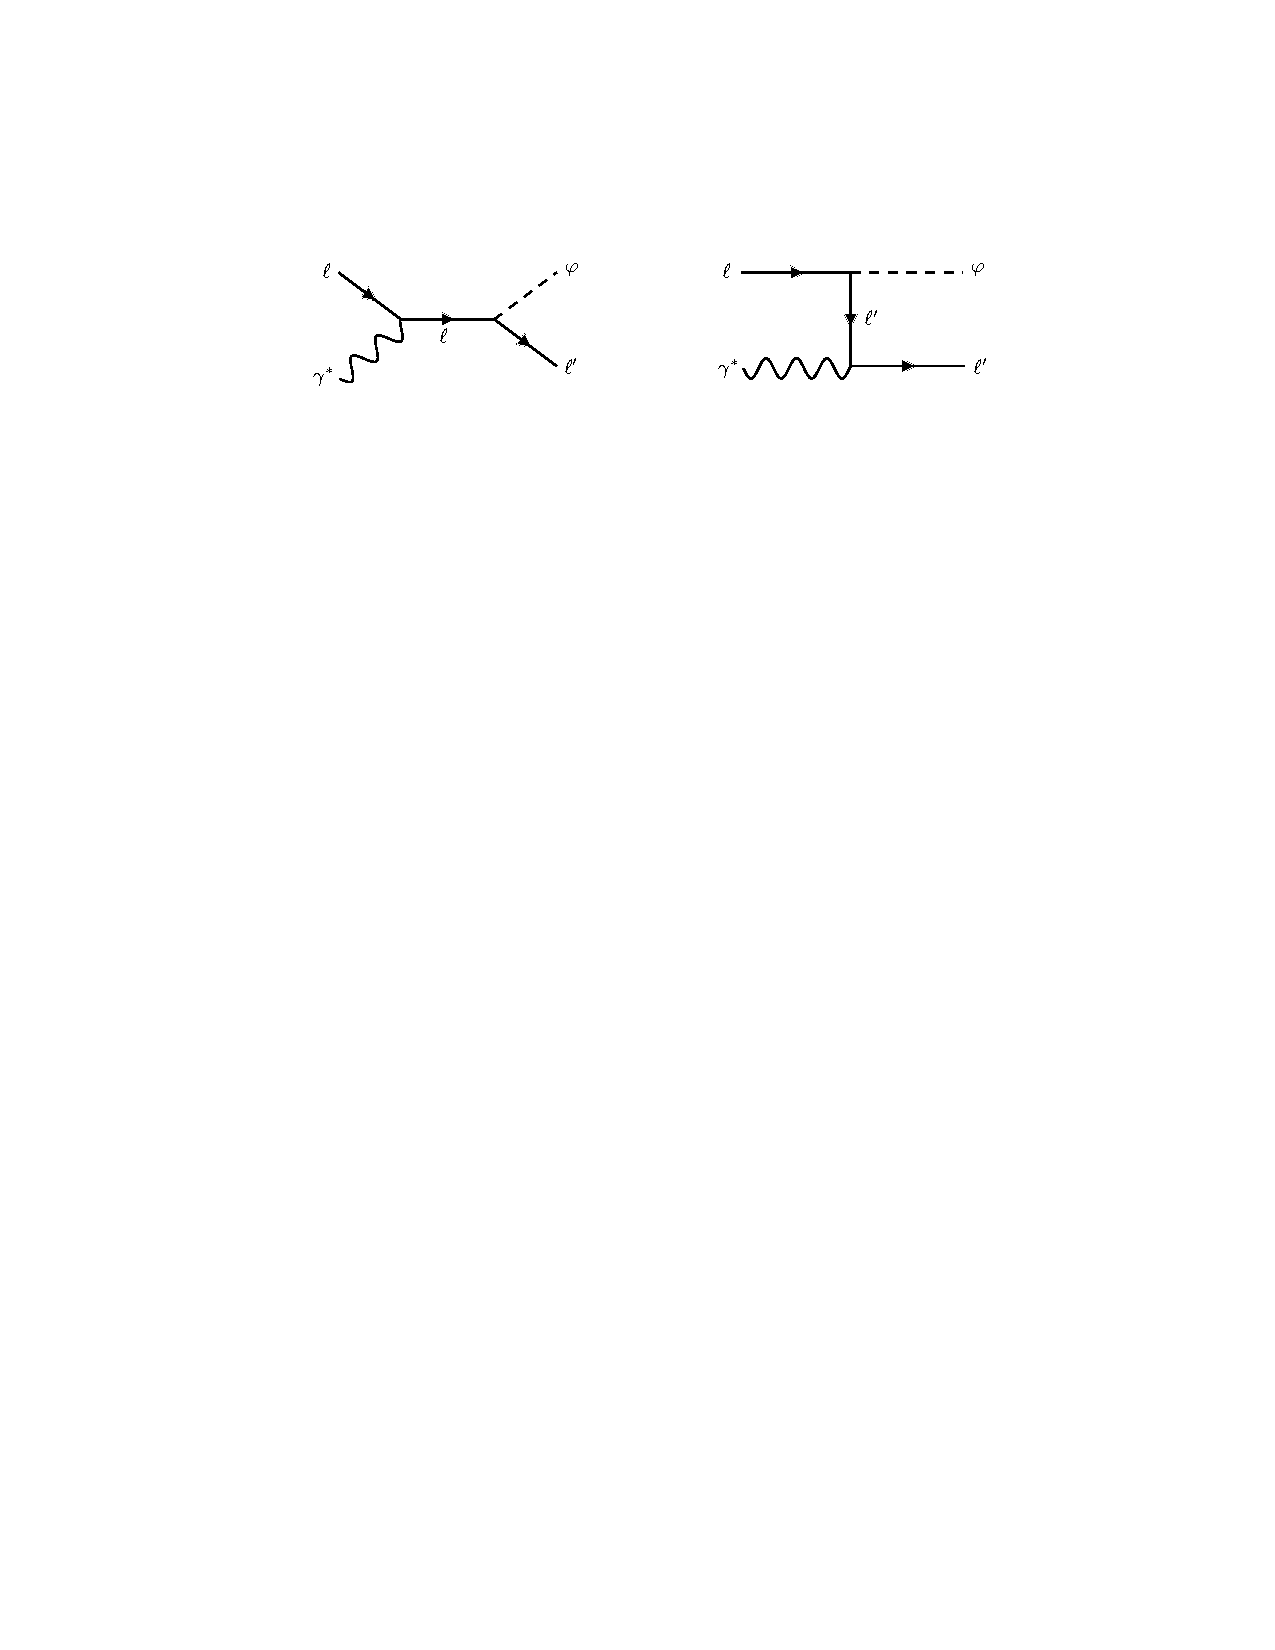
\includegraphics[width=\linewidth]{figures/chapter4/WW_diagrams.pdf}
    \caption{Relevant $2\rightarrow 2$ Feynman diagrams for approximating the process $\ell A_Z \rightarrow \ell' A_Z \varphi$ via the Weizs\"acker-Williams approximation.}
    \label{fig:WW_diagrams}
\end{figure}
where the Dirac-vertices $\Gamma$ for (pseudo)-scalars and (axial)-vectors are the same as those in Eqs.~\ref{eq:scalar_vertex}-\ref{eq:vector_vertex}. Averaging over the square of the amplitude yields
\begin{align}
    \overline{|{\cal M}^{2\rightarrow 2}|^2} &= g^2 e^4 \overline{|{\cal A}^{2\rightarrow 2}|^2}.
\end{align}
Similarly to the $2\rightarrow 3$ process, the amplitude can be decomposed into a PC and PV piece, $|{\cal A}^{2\rightarrow 2}|^2 = |{\cal A}_0^{2\rightarrow 2}|^2 + \sin^2{\theta}|{\cal A}_{\rm PV}^{2\rightarrow 2}|^2$. For scalars, $|{\cal A}^{2\rightarrow2}|^2$ is given by

\begin{align}
    \overline{|{\cal A}_{S,0}^{2\rightarrow2}|^2} &= -\frac{(s+u)^2}{su} + 2(m_\varphi^2 - (m_\ell + m_{\ell'})^2)\frac{s+u}{su}\left(1+\frac{m_\ell^2}{s}+\frac{m_{\ell'}^2}{u}-\frac{m_\varphi^2}{s+u}\right),\nonumber\\
    \overline{|{\cal A}_{S,{\rm PV}}^{2\rightarrow2}|^2} &= 8m_\ell m_{\ell'}\frac{s+u}{su}\left(1+\frac{m_\ell^2}{s}+\frac{m_{\ell'}^2}{u}-\frac{m_\varphi^2}{s+u}\right).\label{eq:scalar_amplitudes_2_2}
\end{align}
Whereas for vectors,
\begin{align}
    \overline{|{\cal A}_{V,0}^{2\rightarrow2}|^2} &= -\frac{(s+u)^2}{su}\left(2+\frac{\Delta m_{\ell\ell'}^2}{m_\varphi^2}\right) + 4\nonumber\\
    &\ \ + 2\left(1-\frac{\Delta m_{\ell\ell'}^2}{m_\varphi^2}\right)(2m_\varphi^2 + (m_\ell + m_{\ell'})^2)\frac{s+u}{su}\left(1+\frac{m_\ell^2}{s}+\frac{m_{\ell'}^2}{u}-\frac{m_\varphi^2}{s+u}\right),\nonumber\\
    \overline{|{\cal A}_{V,{\rm PV}}^{2\rightarrow2}|^2} &= -\frac{4m_\ell m_{\ell'}}{m_\varphi^2}\left[\frac{(s+u)^2}{su}+3m_\varphi^2\frac{s+u}{su}\left(1+\frac{m_\ell^2}{s}+\frac{m_{\ell'}^2}{u}-\frac{m_\varphi^2}{s+u}\right)\right].\label{eq:vector_amplitudes_2_2}
\end{align}
To evaluate at $t = t_-$, we note that the only dependence on $t$ is in $s$  (Eq.~\ref{eq:s}). At $t = t_-$, $\cos{\theta_k^0} = \pm 1$, so 
\begin{align}
    s|_{t=t_-} &= -\left(1+\frac{E}{M}\right)t_- \pm \frac{2Q_-}{V}|{\bf p}|[|{\bf p}| - |{\bf k}|\cos{\theta_k}].
\end{align}
Numerically, we find that $\left.\cos{\theta_q^0}\right|_{t=t_-}$ is usually $-1$, which is what one would expect if the lepton and photon collided head-on. 

\subsection{Improved Weizs\"acker-Williams Approximation}\label{sec:IWW}
In the {\it Improved}\footnote{It is so-called not due to an increase in accuracy of the approximation, but to a decrease in computational complexity.} Weizs\"acker-Williams approximation (as defined in Ref. \cite{Kim:1973he}), the effective photon flux $\chi$ is additionally simplified to be independent of $E_k$ and $\theta_k$. To accomplish this, we take $t_- = [((m_\ell + m_\varphi)^2 - m_{\ell'}^2)/2E]^2$ and $t_+ = 4ME^2/(2E+M)$ in the bounds of integration. Other references take $t_+ = m_\ell^2 + m_\varphi^2$ which is likely sufficient to capture most of the dependence of the form-factor, but we note Eqs.~\ref{eq:t_+}-\ref{eq:t_-} implies $t_+t_- = M^2u^2/[(E-E_k+M)^2-V^2]$, which in the appropriate limit gives our value of $t_+$ above as an absolute upper-bound on $t$. Given the behavior of $F(t)^2/t^2$ for large $t$, we expect the difference between these $t_+$ to be inconsequential.

While we stop at this point in our analysis when computing the differential cross-sections in the Improved Weizs\"acker-Williams approximation, there are additional approximations one can make to perform the angular integral, resulting in an approximation for $d\sigma/dE_k$. In particular, if $m_\ell/E, m_{\ell'}/E,m_\varphi/E, \theta_k \ll 1$ and $t \sim t_-$, then one can approximate
\begin{align}
    s &\approx -\frac{u}{1-x}\\
    u &\approx (1-x)m_\ell^2-m_{\ell'}^2-(1-1/x)m_\varphi^2 - x \theta_k^2E^2\\
    t_{-} &\approx \frac{u^2}{4(1-x)^2E^2}
\end{align}
inside the $2\rightarrow 2$ amplitudes in Eqs. \ref{eq:scalar_amplitudes_2_2} and \ref{eq:vector_amplitudes_2_2}. With everything expressed in terms of $u$, the integral over $\theta_k$ can be replaced with an integral over $u$ with $du \approx -2x\theta_k E^2d\theta_k \approx -2xE^2\sin{\theta_k} d\theta_k$. Then we have
\begin{align}
    \left(\frac{d\sigma}{dE_k}\right)_{\it IWW} &= \frac{g^2}{8\pi}\alpha^2 \chi \int_{\theta_{\rm min}}^{\theta_{\rm max}}{d\theta_k\,\sin{\theta_k} \frac{|{\bf k}|}{|{\bf p}|V}\frac{1}{t_-}\left|{\cal A}^{2\rightarrow 2}\right|^2_{t=t_-}}\nonumber\\
    &= \frac{g^2}{4\pi\alpha^2}\chi\frac{|{\bf k}|}{E^2}\frac{1-x}{x}\int_{u_{\rm min}}^{u_{\rm max}}{\frac{du}{u^2} \left|{\cal A}^{2\rightarrow 2}\right|^2_{t=t_-}}.\label{eq:IWW}
\end{align}
Finally, assuming that $\theta_k$ becomes large enough that $\theta_k E^2 \gg m_\ell^2,m_{\ell'}^2,m_\varphi^2$, we can take $u_{\rm min} = -\infty$, and keep $u_{\rm max} = (1-x)m_\ell^2 + (1-1/x)m_\varphi^2 - m_{\ell'}^2  - x\theta_{\rm min}^2E^2$. While for beam-dump or fixed-target experiments, $\theta_{\rm min}$ is often zero, $\theta_{\rm min}$ is set by the detector geometry for lepton-ion colliders.

For completion, we evaluate the integral over $du$ in  Eq.~\ref{eq:IWW} for the terms that appear in $|{\cal A}^{2\rightarrow }|^2_{t = t_-}$ for both scalars and vectors. In particular, we have
\begin{align}
    \int_{-\infty}^{u_{\rm max}}{\frac{du}{u^2}}\left[-\frac{(s+u)^2}{su}\right] &\approx -\frac{x^2}{1-x}\frac{1}{u_{\rm max}}\\
    \int_{-\infty}^{u_{\rm max}}{\frac{du}{u^2}}\frac{s+u}{su}\left[1+\frac{m_\ell^2}{s}+\frac{m_{\ell'}^2}{u}-\frac{m_\varphi^2}{s+u}\right] &\approx -\frac{x(u_{\rm max} - 2x\theta_{\rm min}^2 E^2)}{6u_{\rm max}^3}
\end{align}

It is straightforward to combine these results with Eqs.~\ref{eq:scalar_amplitudes_2_2} and \ref{eq:vector_amplitudes_2_2} to find approximate expressions for $d\sigma/dE_k$. We do not compare these formulae to the exact cross-sections $d\sigma/dE_k$, as we are more interested in the lab-frame differential cross-sections. For analysis of these approximate differential cross-sections in the context of beam-dump experiments, we again refer to Refs.~\cite{Liu:2016mqv,Liu:2017htz,Chen:2017awl}.
\subsection{Cross-Section Comparisons}\label{sec:cx_comparison}

To test the validity of the WW and IWW approximations, we can plot the exact and approximate cross-sections (along with the relative error) for a variety of processes and colliders. For simplicity, we focus on two cases: the diagonal process $\ell A_Z \longrightarrow \ell A_Z \varphi$, and the off-diagonal process $\ell A_Z \longrightarrow \tau A_Z \varphi$. In either case, we allow the interaction to be scalar-like or vector-like with arbitrary parity violation. The results for each process are shown in Fig.~\ref{fig:WW_diagonal} and Fig.~\ref{fig:WW_tau}, respectively.

First, we focus on the diagonal process shown in Fig.~\ref{fig:WW_diagonal}. These are most directly comparable to the results from Refs.~\cite{Liu:2016mqv,Liu:2017htz,Chen:2017awl}, although those references compare the differential cross-section $d\sigma/dx$ w.r.t. $x = E_k/E$. For the diagonal case, we find excellent agreement between the WW approximation and exact result for almost all range of masses, with better agreement for higher lepton beam energy. In particular, there are ${\cal O}(1)$ deviations for E137 at small masses, but otherwise the EIC approximation agrees with the exact result to within $10\%$ at small masses and within $1\%$ at large masses. The agreement for the muon beam experiments is even better, with an agreement of within $1\%$ or less across the total range of masses considered. We also find very good agreement with the IWW approximation, with only $O(1)$ deviations at large masses. In particular, the agreement we find between the IWW and exact methods is better than is found in Refs.~\cite{Liu:2016mqv,Liu:2017htz}, even for E137. This is likely due to the fact that while we assume $t_{\pm}$ are independent of $E_k$ and $\theta_k$ in the bounds of the $t$ integral to simplify the photon flux, we do not employ the additional approximation for the angular integral described in Section~\ref{sec:IWW}. 
\clearpage
\begin{figure}[t!]
    \centering
    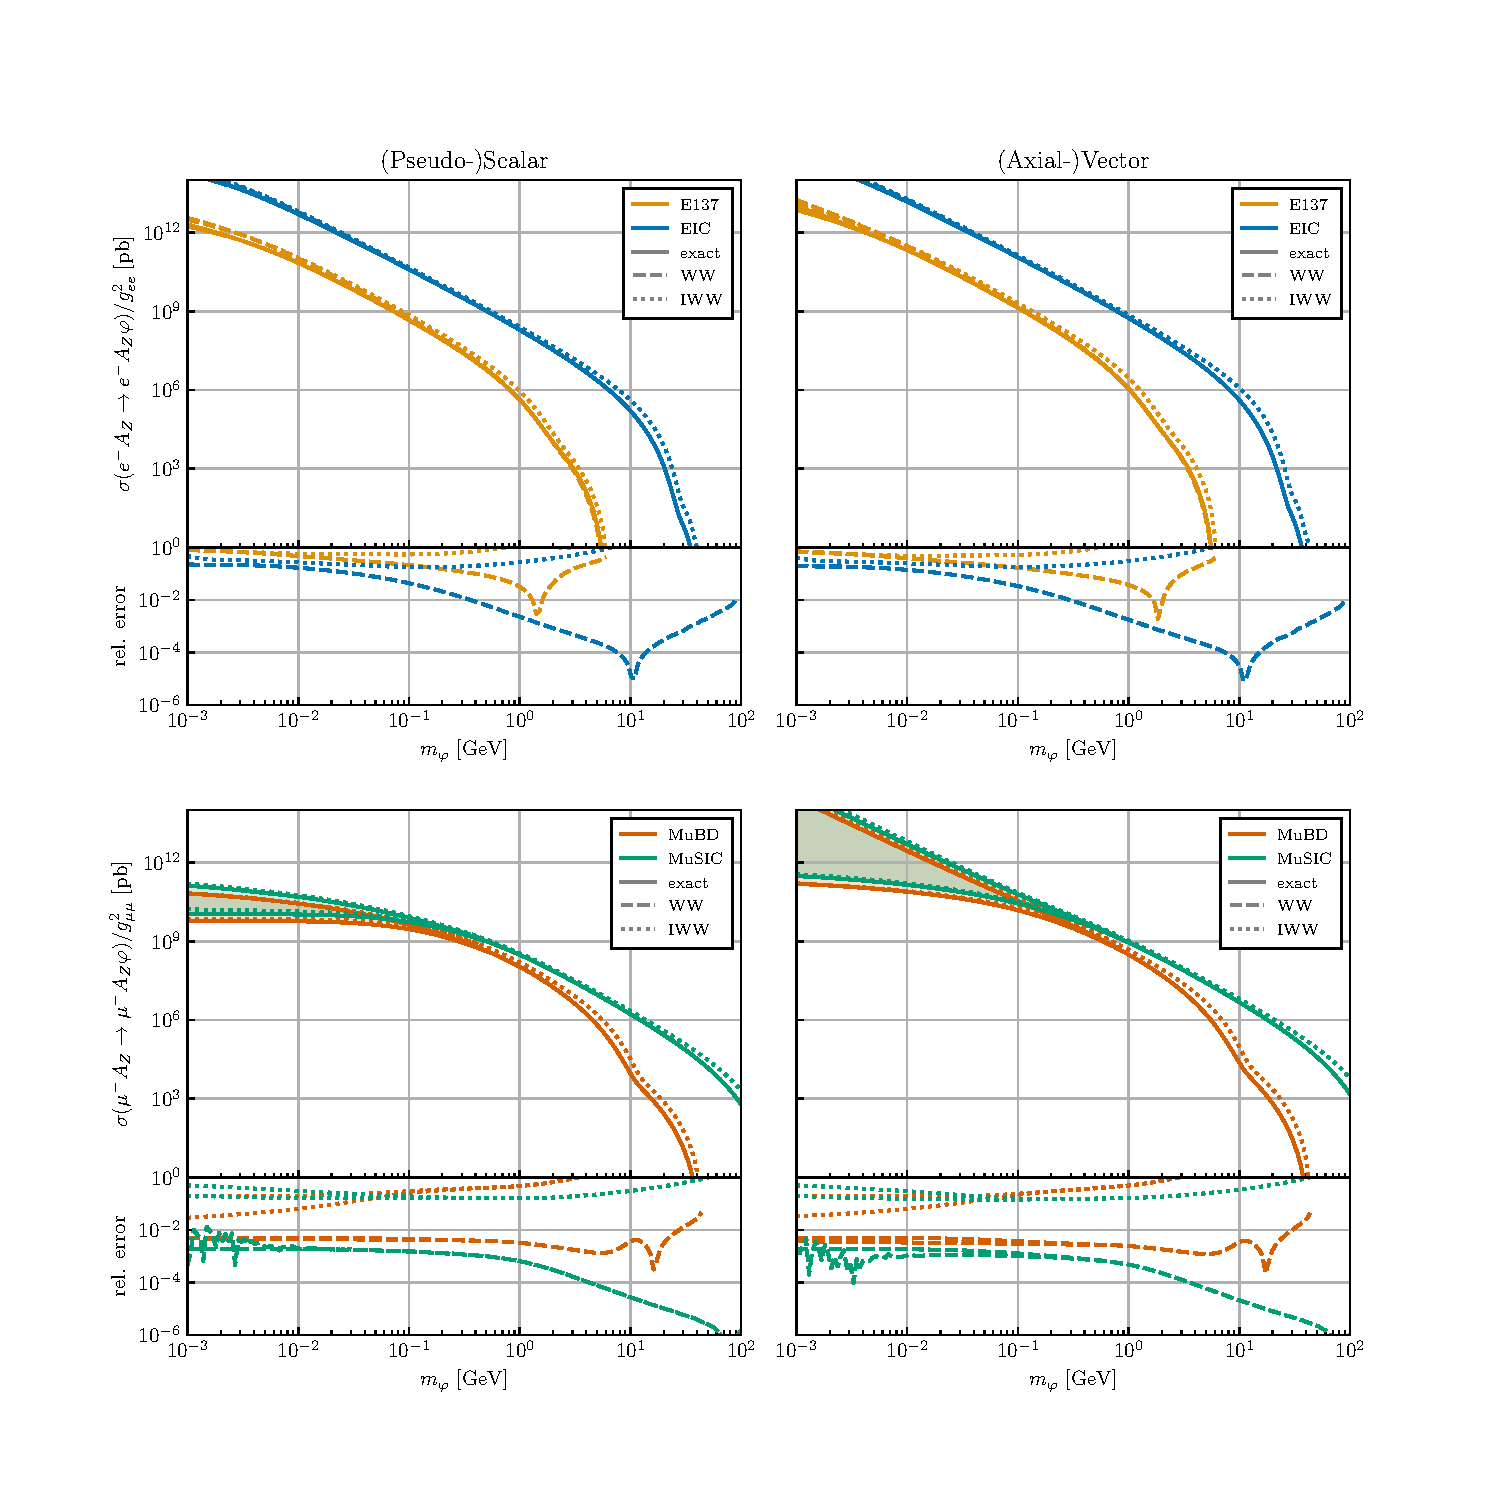
\includegraphics[trim={2.5cm 0 2.5cm 0}, width=0.9\linewidth]{figures/chapter4/crossx_approximations_diagonal.pdf}
    \caption[Comparisons between cross-sections computed exactly and via the Weiz\"acker-Williams and Improved Weizs\"acker-Williams approximations for the process $\ell A_Z \rightarrow \ell A_Z \varphi$ at various lepton-nucleus collision experiments.]{Comparisons between exact (solid) and approximate (``WW,'' dashed and ``IWW,'' dotted) cross-sections, along with relative errors (bottom of each plot), for some lepton-nucleus collisions. The plots on the top compare the approximate and exact cross-sections for the electron-nucleus collisions at E137 and the EIC, whereas the plots on the bottom compare the approximate and exact cross-sections for the muon-nucleus collisions at the hypothetical $1~{\rm TeV}$ MuBeD and MuSIC (defined in the text). The plots on the left compare the results for (pseudo)-scalars, while the plots on the right compare the results for (axial)-vectors. }
    \label{fig:WW_diagonal}
\end{figure}
\clearpage
\begin{figure}[t!]
    \centering
    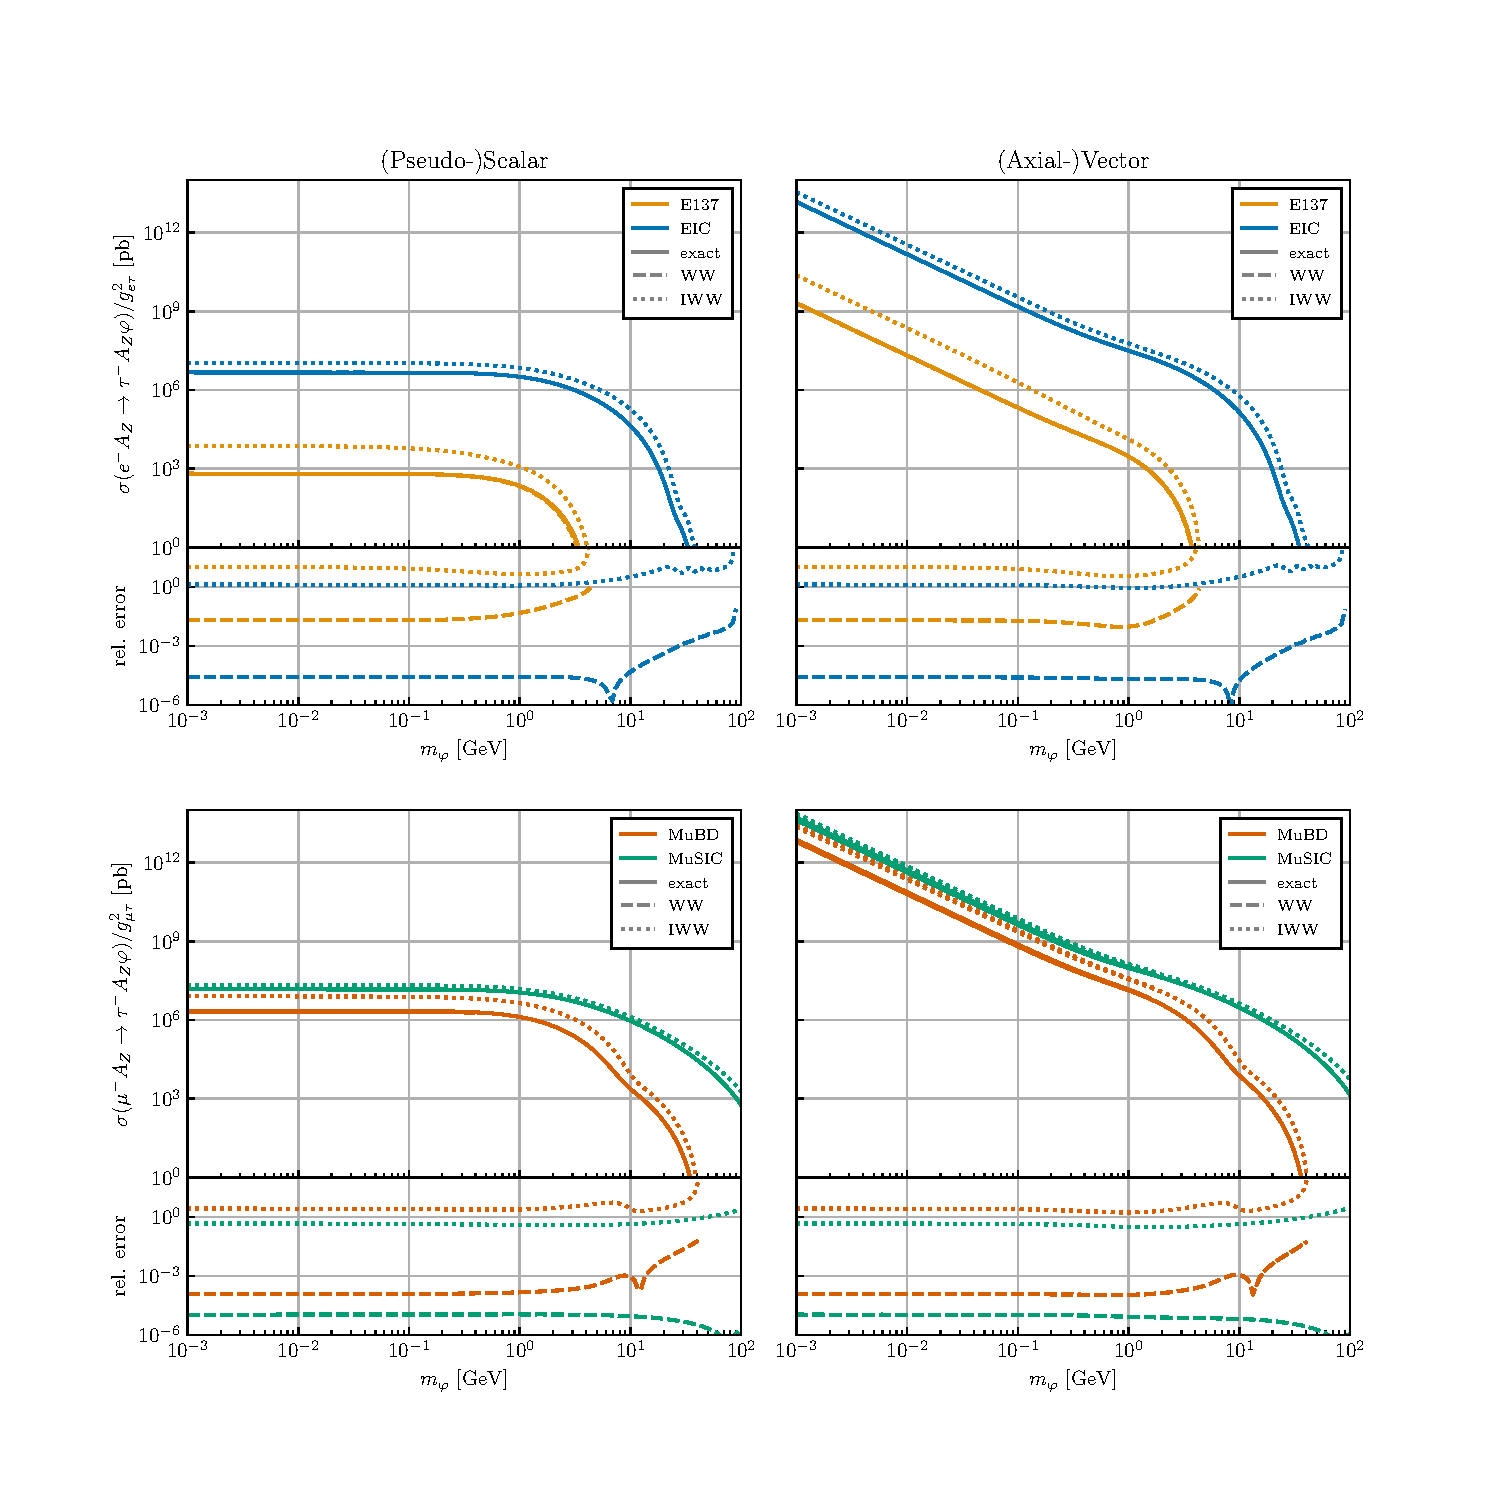
\includegraphics[trim={2.5cm 0 2.5cm 0}, width=0.9\linewidth]{figures/chapter4/crossx_approximations_tau.pdf}
    \caption[Comparisons between cross-sections computed exactly and via the Weiz\"acker-Williams and Improved Weizs\"acker-Williams approximations for the process $\ell A_Z \rightarrow \tau A_Z \varphi$ at various lepton-nucleus collision experiments.]{Comparisons between exact (solid) and approximate (``WW,'' dashed and ``IWW,'' dotted) cross-sections, along with relative errors (bottom of each plot), for some lepton-nucleus collisions. The plots on the top compare the approximate and exact cross-sections for the electron-nucleus collisions at E137 and the EIC, whereas the plots on the bottom compare the approximate and exact cross-sections for the muon-nucleus collisions at the hypothetical $1~{\rm TeV}$ MuBeD and MuSIC (defined in the text). The plots on the left compare the results for (pseudo)-scalars, while the plots on the right compare the results for (axial)-vectors. }
    \label{fig:WW_tau}
\end{figure}
\clearpage


Given that the analyses in the literature focus on the diagonal case, it is worth considering whether the WW approximations still apply for LFV particle production. In Fig.~\ref{fig:WW_tau}, we consider the LFV $\ell$-$\tau$-conversion process $\ell^- A_Z \rightarrow \ell'^- A_Z \varphi$ for $\varphi$.  Once again, we find excellent agreement between the WW approximation and the exact result, especially at higher lepton beam energies. In particular, the WW approximation is accurate to within $1\%$ for E137, $0.01\%$ for the EIC and MuBeD, and $0.001\%$ for MuSIC. The IWW also fares well for the EIC and MuSIC, with a disagreement of at most a factor of 2 for most masses. However, it performs slightly worse for the beam dump experiments E137 and MuBeD, disagreeing by a factor of few (although no more than 10) over the masses considered.

\section{Kinematical Distributions of $\varphi$}\label{sec:phi_kin}
In the preceding sections, we have examined the total production cross-section for various lepton beam-dump experiments and lepton-ion colliders. However, the signal cross-section is often much smaller, as the particle must decay to visible and identifiable products within or near a detector. Hence, particles that are extremely boosted can evade detection by decaying far from the experimental apparatus, and (particularly for the lepton-ion collision case) particles that are produced too far forward or backward may escape along the beam axis. Hence, in order to better compare lepton-beam dump and lepton-ion collider scenarios, it is important to examine the kinematic distributions of the final-state particles as well. 

It is straightforward to derive the kinematic distributions of $\varphi$ from the differential cross-section \ref{eq:dsig}. In particular, the energy-angle distribution for the final-state particle $\varphi$ in the nucleus frame is given by 
\begin{align}
    \rho_{E,\theta}(E_\varphi, \theta_\varphi) &= \frac{1}{\sigma}\frac{\partial \sigma}{\partial E_\varphi \,\partial\theta_\varphi}(E_\varphi, \theta_\varphi). \label{eq:phi_dist}
\end{align}
This is all well and good in beam-dump and fixed-target experiments, for which the frame of the nucleus is the same as the frame of the lab, but surely must fail for an ion moving close to the speed of light relative to the lab. Indeed, labeling those variables in the ion rest frame `ion' and those in the lab frame `lab', one has to perform a coordinate transformation 
\begin{align}
    \frac{1}{\sigma}\frac{\partial \sigma}{\partial E^{\rm lab}\,\partial \theta^{\rm lab}} = \frac{1}{\sigma}\frac{\partial(E^{\rm ion}, \theta^{\rm ion})}{\partial(E^{\rm lab}, \theta^{\rm lab})}\frac{\partial \sigma}{\partial E^{\rm ion} \partial\theta^{\rm ion}}.
\end{align}
Surprisingly, it turns out that 
\begin{align}
    \frac{\partial(E^{\rm ion}, \theta^{\rm ion})}{\partial(E^{\rm lab}, \theta^{\rm lab})} = 1.
\end{align}
This can be verified through explicit computation using Eqs.~\ref{eq:E_transform}-\ref{eq:theta_transform} below, but can also be understood by examining the Lorentz-invariant measure $\delta(p^2 - m^2)d^4p$. We can expand the four-momentum $p^2 = E^2 - |{\bf p}|^2$ and the integration measure $d^4p = |{\bf p}|^2\sin{\theta}dE\,d|{\bf p}|\,d\theta\,d\phi$, where $\theta$ is the momentum angle with-respect-to the beam axis and $\phi$ is the transverse angle. With this in mind, we have
\begin{align}
    \delta(E^2-|{\bf p}|^2 - m^2)|{\bf p}|^2\sin{\theta}dE\,d|{\bf p}|\,d\theta\,d\phi &= \frac{\delta(|{\bf p}| - \sqrt{E^2 - m^2})}{2|{\bf p}|}|{\bf p}|^2 \sin{\theta}dE\,d|{\bf p}|d\theta\,d\phi\nonumber\\
    &= \frac{1}{2}\sqrt{E^2 - m^2}\sin{\theta}\,dE\,d\theta\,d\phi\nonumber\\
    &= \frac{1}{2}[|{\bf p}_{\perp}|d\phi][dE\,d\theta].
\end{align}
In the last line, we have identified $\sqrt{E^2 - m^2}\sin{\theta}\equiv |{\bf p}_\perp|$ and split the measure into two terms. The first term, $|{\bf p}_\perp|\,d\phi$, is invariant under boosts along the beam-axis because $ {\bf p}_\perp' = {\bf p}_\perp$ and $\phi'=\phi$ under these transformations. The left-hand-side is manifestly Lorentz-invariant, and so is also invariant under boosts along the beam-axis. Hence, it must be the case that the remaining measure, $dE\,d\theta$, is also invariant under boosts along the beam-axis.\footnote{While we have proven this for a Lorentz-invariant measure, we note that the same derivation applies to the Galilean-invariant measure with $\delta(E^2 - |{\bf p}|^2 - m^2) \rightarrow \delta(E - |{\bf p}|^2/2m)$.} With this useful fact, the $E$-$\theta$ kinematic distribution in the lab frame is indeed given by
\begin{align}
    \rho(E_\varphi^{\rm lab}, \theta_\varphi^{\rm lab}) &= \frac{1}{\sigma}\frac{\partial \sigma}{\partial E_\varphi^{\rm ion} \,\partial\theta_\varphi^{\rm ion}}(E_\varphi^{\rm ion}, \theta_\varphi^{\rm ion})
\end{align}
without an associated Jacobian factor. While this is not a massive conceptual shift, it does simplify numerical evaluation of the distributions substantially. One simply needs the expressions for $E^{\rm ion}$ and $\theta^{\rm ion}$ in terms of $E^{\rm lab}$ and $\theta^{\rm lab}$. These are
\begin{align}
    E_\varphi^{\rm ion} &= \gamma_{\rm ion}\left(E_\varphi^{\rm lab} + v_{\rm ion} |{\bf k}^{\rm lab}_\varphi|\cos{\theta_\varphi^{\rm lab}}\right)\label{eq:E_transform}\\
    \tan{\theta_\varphi^{\rm ion}} &= \frac{\sin{\theta_\varphi^{\rm lab}}}{\gamma_{\rm ion}\left(\cos{\theta_\varphi^{\rm lab}} + v_{\rm ion}/v_\varphi^{\rm lab}\right)}\label{eq:theta_transform}.
\end{align}
where $v_{\rm ion}$ is the speed of the ion in the lab frame and $\gamma_{\rm ion} = 1/\sqrt{1-v_{\rm ion}^2}$ its boost. In lab settings, it is often preferable to speak in terms of the boost $\gamma_\varphi^{\rm lab} = E_\varphi^{\rm lab}/m_\varphi$ and the pseudorapidity $\eta_{\varphi}^{\rm lab} = -\log{\tan{(\theta_\varphi^{\rm lab}/2)}}$. The former is useful for considering the decay lengths of particles in the lab, and the latter is convenient when describing a detector's ability to identify signals on either side of the interaction vertex. In particular, in collider experiments, particles with large $|\eta|$ may escape along the beam-pipe.

\subsection{Pseudorapidity Distributions for Beam Dump vs. Collider Experiments}\label{sec:phi_eta}
The pseudorapidity distribution for the particle $\varphi$ can be obtained from Eq.~\ref{eq:phi_dist} by integrating over $dE$ and multiplying by the Jacobian $|d\theta/d\eta|$:
\begin{align}
    \rho_\eta(\eta) &= \int{dE\, \rho_{E,\theta}(E, \theta(\eta))}\left|\frac{d\theta}{d\eta}\right| \nonumber\\
    &= \int{dE\,\rho_{E,\theta}(E,2\arctan{e^{-\eta}})}\,{\rm sech}{\,\eta}.
\end{align}
\begin{figure}[t!]
    \centering
    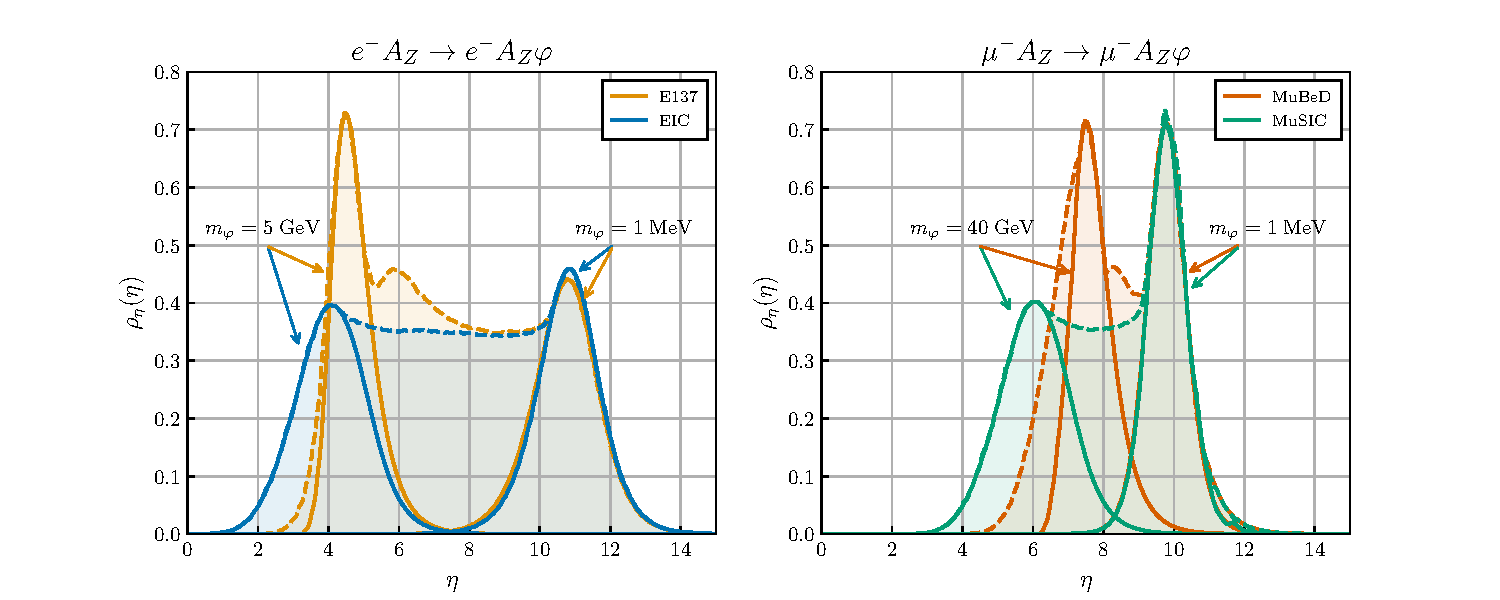
\includegraphics[width=\linewidth]{figures/chapter4/eta_distributions_diagonal.pdf}
    \caption[Pseudo-rapidity distributions of scalars produced at various lepton-nucleus collision experiments.]{A plot illustrating the range of pseudorapidity distributions at E137, the EIC, MuBeD and MuSIC. For the electron beam experiments, the distributions are swept from $m_\varphi=1~{\rm MeV}$ to $m_\varphi = 5~{\rm GeV}$, whereas for the muon beam experiments, the distributions are swept from $m_\varphi=1~{\rm MeV}$ to $m_\varphi = 40~{\rm GeV}$. The envelope of all such distributions is plotted with a dashed line and shaded in, with the nedpoint distributions plotted in solid.}    \label{fig:eta_distributions_diagonal}
\end{figure}
Equipped with this result, we can compare the distributions at different experiments. To begin, we examine the distributions for the diagonal interaction $\ell A_Z \rightarrow \ell A_Z\varphi$ with a PC scalar. To get a sense of the distributions over a large range of masses, we fill in the envelope of all distributions between a minimum and maximum $m_\varphi$, and then plot the endpoints in solid. For the electron beam experiments, we plot over the range $m_\varphi = 1~{\rm MeV}$ to $m_{\varphi} = 5~{\rm GeV}$, whereas for the muon beam experiments we plot over the range $m_\varphi = 1~{\rm MeV}$ to $m_{\varphi} = 40~{\rm GeV}$. The results are shown in Fig.~\ref{fig:eta_distributions_diagonal}. For low masses, it appears that there is little difference between the distributions at the lepton-ion colliders and their beam-dump counterparts, but deviations become significant at higher masses. 

It is important to put these distributions into the context of the detector apparatus at each experiment. Beam-dump experiments typically have detectors along the beam axis far past the target, so they should in principle have no difficulty capturing forward-produced (high $\eta$) particles. The EIC and MuSIC, however, are collider experiments, so particles with high pseudorapidity can escape down the beam-pipe undetected, unless a dedicated forward or backward detector apparatus is constructed. In particular, the pseudo-rapidity range on the electron-side of the EIC is expected to be $|\eta| < 3.5$ \cite{AbdulKhalek:2021gbh}. Based on the left panel of Fig.~\ref{fig:eta_distributions_diagonal}, we see that for $m_\varphi \lesssim 5~{\rm GeV}$, most particles will have a an average pseudo-rapidity $|\overline{\eta}| > 4$, and hence only a small fraction of such particles will have the potential to be detected at the EIC. In  Chapter~\ref{bosons}, we will explore the possibility of capturing such forward-produced particles with the addition of a ``far backward'' detector, with a tracking module at $z \approx 6~{\rm m}$ from the interaction point (similar to the planned B0 spectrometer on the ion side of ePIC detector \cite{Adkins:2022jfp}). In the right panel of Fig.~\ref{fig:eta_distributions_diagonal}, we see that the average pseudorapidity at MuSIC is even higher, with $|\overline{\eta}| \gtrsim 6$ for $m_\varphi < 40~{\rm GeV}$. Although no concrete pseudo-rapidity requirement has currently been proposed for MuSIC, higher pseudo-rapidity resolution would require detectors far down the beam-pipe. Hence, one can expect that for light masses, the EIC and MuSIC will be out-performed by the corresponding beam-dumps E137 and MuBeD, while these lepton-ion colliders will have the advantage in the heavy-mass regime.

\begin{figure}[t!]
    \centering
    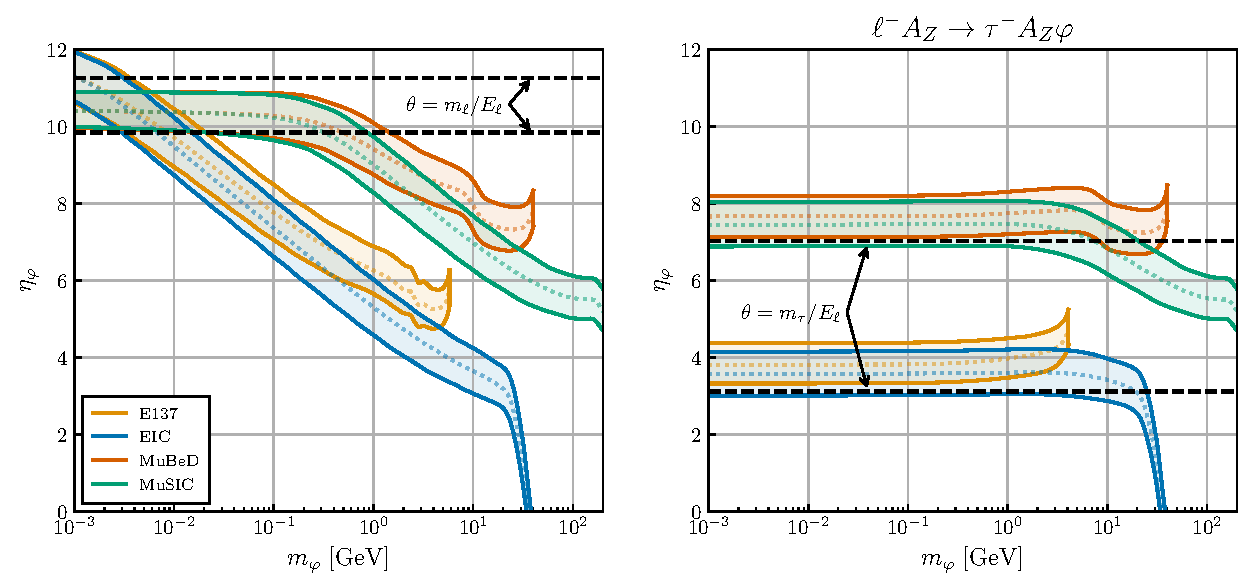
\includegraphics[width=\linewidth]{figures/chapter4/median_eta.pdf}
    \caption[Interquartile range as a function of mass for pseudo-rapidity distributions of scalars produced at various lepton-nucleus collision experiments.]{Interquartile range of $\eta$ as a function of mass for on-diagonal production of a $\varphi$ (left) and production of a $\varphi$ via $\tau$-conversion (right). The dashed lines represent the opening angle in the limit of small mass, which is roughly $\theta \approx m_{\ell'}/E_\ell$, or $\eta \approx \log{(2E_\ell/m_{\ell'})}$.}
    \label{fig:pseudorapidity_IQR}
\end{figure}

To better visualize the pseudo-rapidity distributions at these experiments, we can plot the interquartile range of the pseudo-rapidity $\eta$ as a function of masses. This is shown for both the diagonal case, as well as the $\tau$-conversion case $\ell A_Z \rightarrow \tau A_Z\varphi$ , in Fig.~\ref{fig:pseudorapidity_IQR}. For these experiments, it appears the angle of the $\varphi$ asymptotes near $\theta = m_{\ell'}/E_\ell$, where $m_{\ell'}$ is the mass of the final-state lepton and $E_\ell$ is the energy of the initial-state lepton in the lab frame. For the EIC, we see that in the diagonal production case, only heavy particles fall within the $|\eta| < 3.5$ pseudo-rapidity requirement, while for the off-diagonal $\tau$ conversion case, a substantial portion of all particles fall within the $|\eta| < 3.5$ case. For MuSIC, on the other hand, almost all particles in both cases lie far beyond the EIC's pseudorapidity requirement. We expect that higher pseudo-rapidities are a generic feature of such a collider due to the much larger inertia of the incident muons, so in the event such a detector is created, additional instrumentation will be included to cover a range of pseudorapidities at least up to $|\eta| < 6$.

As discussed previously, higher pseudo-rapidities are not a problem at beam dump experiments, so these experiments should in principle be able to detect the decay products of all particles $\varphi$ produced in this fashion. The only caveat is that these particles (especially the lighter ones) are often produced with a very high boost, so it is possible depending on their coupling that they decay far beyond the confines of the experiment.

While we have only plotted the PC scalar case here, we do not expect the qualitative features for other particle types to differ, as the particle type does not strongly impact the kinematics of the process. The same can not be said about changing the final-state lepton, as the kinematics of $\varphi$ and the final-state lepton is directly dependent on their relative mass and energy. The processes we have omitted from discussion ($e^- A_Z \rightarrow \mu^- A_Z\varphi$ and $\mu^- \rightarrow e^- A_Z\varphi$) are already very constrained from limits on $\mu \rightarrow e\gamma$ and (for light $\varphi$) $\mu \rightarrow e+{\rm inv.}$, and are therefore unlikely to have any signal potential at these experiments.

\subsection{Boost Distributions for Beam Dump vs. Collider Experiments}\label{sec:phi_boost}

Similar to before, the boost distribution for the particle $\varphi$ can be obtained from Eq.~\ref{eq:phi_dist} by integrating over $d\theta$ and multiplying by the Jacobian $|dE/d\gamma|$:
\begin{align}
    \rho_\gamma(\gamma) &= \int{d\theta\, \rho_{E,\theta}(E(\gamma), \theta)\left|\frac{dE}{d\gamma}\right|} \nonumber\\
    &= \int{d\theta\,\rho_{E,\theta}(\gamma m_\varphi, \theta)}m_\varphi.
\end{align}
With this, we plot the boost distributions over a range of masses for the process $\ell^- A_Z \rightarrow \ell^- A_Z \varphi$ in Fig.~\ref{fig:boost_distributions_diagonal}.

\begin{figure}[t!]
    \centering
    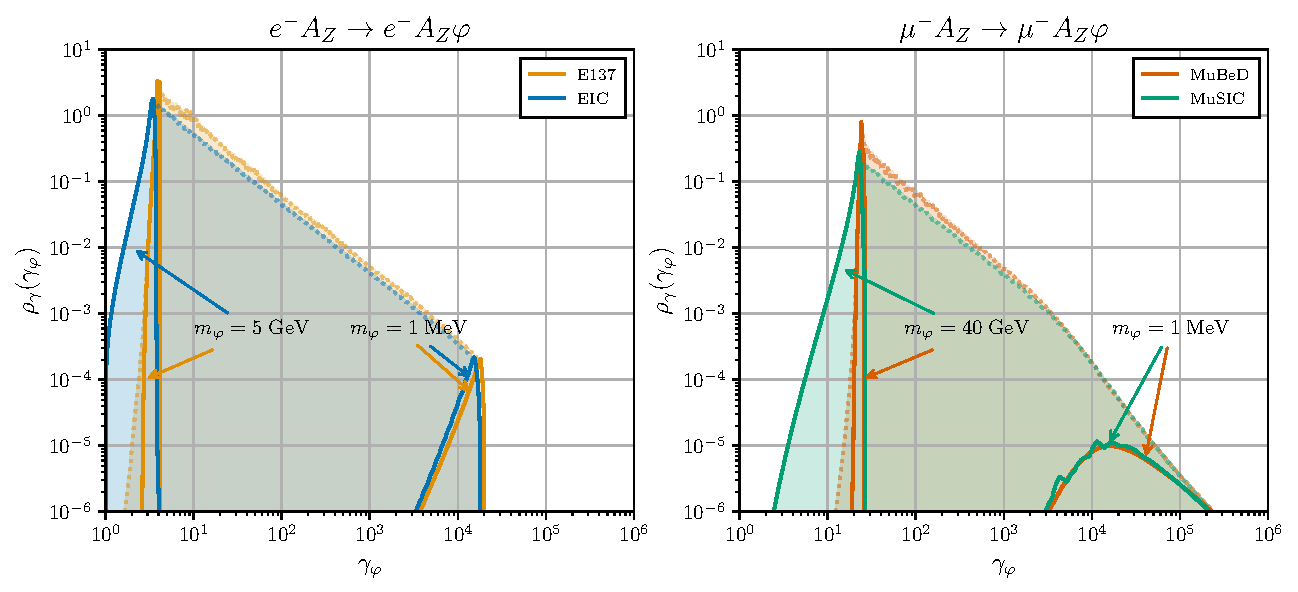
\includegraphics[width=\linewidth]{figures/chapter4/gamma_distributions_diagonal.pdf}
    \caption[Boost distributions of scalars produced at various lepton-nucleus collision experiments.]{A plot illustrating the range of boost distributions at E137 and the EIC (left) and MuBeD and MuSIC (right). For the electron beam experiments, the distributions are swept from $m_\varphi=1~{\rm MeV}$ to $m_\varphi = 5~{\rm GeV}$, whereas for the muon beam experiments, the distributions are swept from $m_\varphi=1~{\rm MeV}$ to $m_\varphi = 40~{\rm GeV}$. The envelope of all such distributions is plotted with a dashed line and shaded in, with the nedpoint distributions plotted in solid.}
    \label{fig:boost_distributions_diagonal}
\end{figure}
We see that not only are light particles produced with very high pseudo-rapidity, but can also have immense boosts as well. In particular, most $1~{\rm MeV}$ particles are produced with upwards of $10^4$ boost, indicating that they will easily escape the detector apparatus before decaying. While the boosts become ${\cal O}(1)$ at E137 and the EIC for GeV-scale ALPs, they are still ${\cal O}(10)$ at MuBeD and MuSIC even up to $m_\varphi = 40~{\rm GeV}$. Notably, despite the additional available energy at the lepton-ion colliders compared to their beam-dump counterparts, the boost distributions (and hence, the energy imparted to the $\varphi$ in the interaction) are almost identical.

Once again, it is instructive to examine the interquartile range of the boost distributions; we do so in Fig.~\ref{fig:boost_IQR} for diagonal production of a $\varphi$ (left) and production of a $\varphi$ via $\tau$-conversion (right). Here, we see that the boost distributions are very narrow, so almost all particles are produced with the same boost, which is quite significant for most masses. It is also clear that for almost the entire range of masses, the boost is near the maximum $\gamma_{\rm max} \approx E_\ell/m_\varphi$.\footnote{Technically, this is not the true maximum, because some energy can be taken from the nucleus as well. However, it is a good approximation for the maximum until $\varphi$ is heavy. } 

One hallmark of particles produced with such a high boost is displaced decay signals. This will be investigated in more detail in Chapter \ref{bosons}, but here we can do some back-of-the-envelope calculations. In particular, if the decay rate of the $\varphi$ is taken to be $\Gamma \approx g^2 m_\varphi / 8\pi$, this corresponds to a decay length of $\gamma c/\Gamma \approx 8\pi E_\ell / g^2 m_\varphi^2$. Typically, displaced decay searches are characterized by a minimum and maximum resolvable displacement, $d_{\rm min}$ and $d_{\rm max}$. Here, $d_{\rm min}$ is set either by the geometry of the detector apparatus or the tracking resolution of the detectors, and $d_{\rm max}$ is set roughly by the overall size of the detector apparatus. Very roughly, given $d_{\rm min}$ and $d_{\rm max}$, we can expect that (so long as the production cross-section is sufficiently large) these experiments will be able to probe mass-coupling products in the range $\sqrt{8\pi E_\ell/d_{\rm max}} \lesssim g m_\varphi \lesssim \sqrt{8\pi E_\ell/d_{\rm min}}$. At the EIC, choosing $d_{\rm min} = 1~{\rm mm}$ and $d_{\rm max} = 1~{\rm m}$, this corresponds to $3\times 10^{-7}~{\rm GeV}\lesssim g m_\varphi \lesssim 10^{-5}~{\rm GeV}$. The parameters of MuBeD are much less certain, but choosing the $E = 1.5~{\rm TeV}$ scenario from Refs.~\cite{Cesarotti:2022ttv,Cesarotti:2023sje} (which has $d_{\rm min} \approx 10~{\rm m}$ and $d_{\rm max}\approx 100~{\rm m}$), we have $2\times 10^{-7}~{\rm GeV}\lesssim g m_\varphi \lesssim 7\times 10^{-7}~{\rm GeV}$. These rough estimates line up well with the more detailed analysis performed in Chapter \ref{bosons}, although the range of accessible parameters is considerably wider, due to the non-zero probability that particles with $c\tau < d_{\rm min}$ or $c\tau > d_{\rm max}$ still decay within the detector.


\begin{figure}[t!]
    \centering
    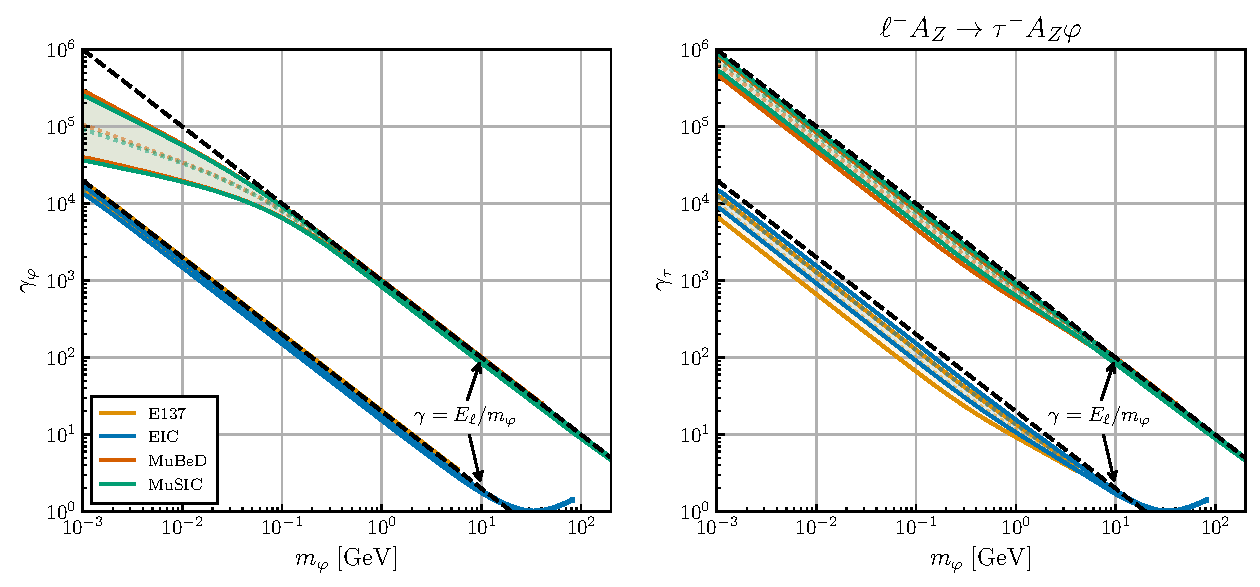
\includegraphics[width=\linewidth]{figures/chapter4/median_gamma.pdf}
    \caption[Interquartile range as a function of mass for boost distributions of scalars produced at various lepton-nucleus collision experiments.]{Interquartile range of $\gamma$ as a function of mass for on-diagonal production of a $\varphi$ (left) and production of a $\varphi$ via $\tau$-conversion. The black dashed lines represent the curve $\gamma = E_\ell/m_\varphi$ for each of the colliders, which is a rough upper-bound which is only exceeded for large $m_\varphi$, when the $\varphi$ must ``borrow'' a significant amount of energy from the nucleus in order to be produced.}
    \label{fig:boost_IQR}
\end{figure}


\section{Kinematical Distribution of Final-State Lepton}\label{sec:l_kin}
Here, we briefly comment on the kinematical distribution of the final-state lepton. In order to obtain this distribution in full generality, one must perform the cross-section integration over $E'$ and $\theta'$ rather than $E_k$ and $\theta_k$. This can be computed by multiplying Eq.~\ref{eq:dsig} {\it within} the $t$-integral by the Jacobian determinant
\begin{align}
    \left|\frac{\partial(E_k,\theta_k)}{\partial(E', \theta')}\right| = \frac{|{\bf p}|'\sin{\theta'}}{|{\bf k}|\cos{\theta_k}} 
    &= \frac{\sqrt{(E - E_k + \frac{t}{2M})^2 - m_f^2 - (E_k^2 - m_\varphi^2)\sin^2{\theta_k}}}{\sqrt{E_k^2 - m_\varphi^2}\cos{\theta_k}}\label{eq:fs_lepton_jacobian}
\end{align}
\begin{figure}[t!]
    \centering
    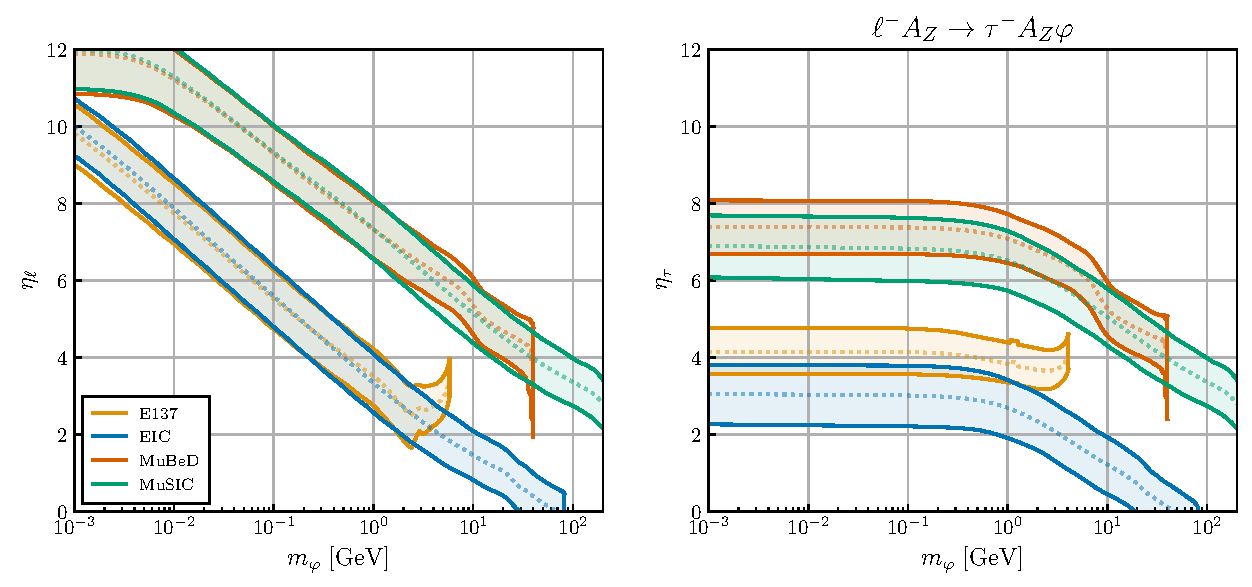
\includegraphics[width=0.9\linewidth]{figures/chapter4/median_eta_lepton.pdf}
    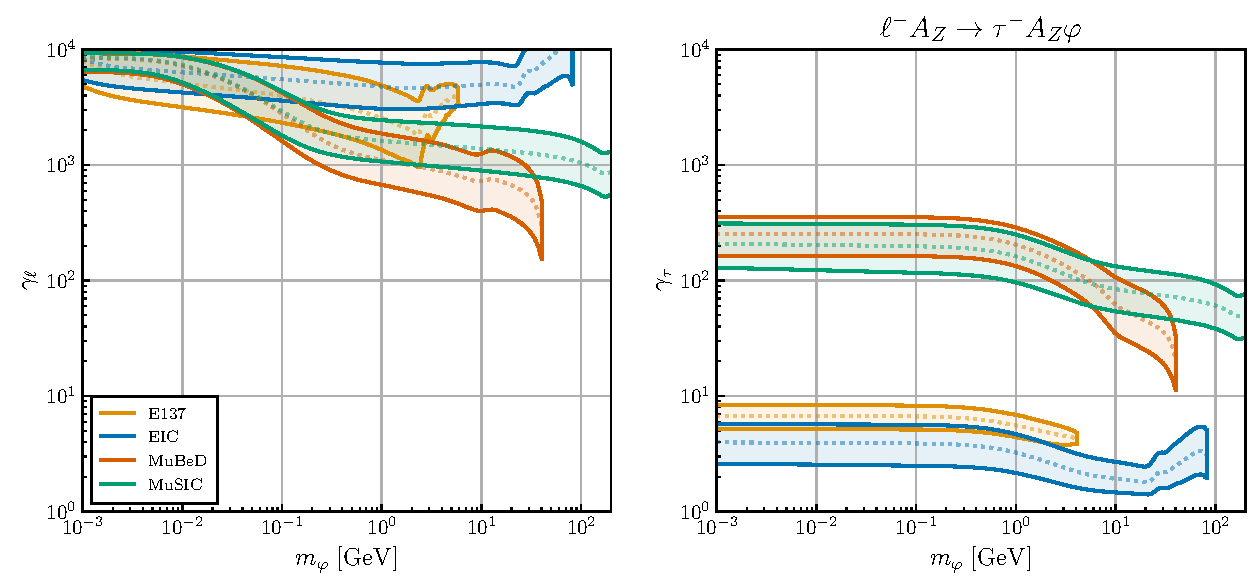
\includegraphics[width=0.9\linewidth]{figures/chapter4/median_gamma_lepton.pdf}
    \caption[Interquartile range as a function of mass for pseudo-rapidity and boost distributions of leptons in certain scalar-production processes at lepton-nucleus collision experiments.]{The interquartile range as a function of mass $m_\varphi$ for the pseudo-rapidity of the final-state lepton (top) and the boost of the final-state lepton (bottom), for both flavor-diagonal (left) and $\tau$-conversion (right) processes.}
    \label{fig:eta_gamma_fs_lepton}
\end{figure}
which will convert $\frac{d\sigma}{dE_kd\theta_k}$ to $\frac{d\sigma}{dE'd\theta'}$. Given the reliability of the WW-approximation, one can obtain an approximation for the distribution by substituting $t = t_{\rm min} \approx \frac{[(m+m_f)^2 - m_i^2]^2}{4E_i^2}$ into Eq.~\ref{eq:fs_lepton_jacobian}. For a rough approximation, one can also perform the limit $\theta_k, m_\varphi/E, m_f/E, \sqrt{t}/E\ll 1$, for which $\left|\partial(E_k,\theta_k)/\partial(E',\theta')\right| \approx E/E_k - 1$. 

Using these formulae, it is possible to examine distributions for the final-state lepton akin to those distributions of the final-state $\varphi$ studied in the previous sections. In Fig.~\ref{fig:eta_gamma_fs_lepton}, we plot the interquartile range for the $\eta$ and $\gamma$ distributions of the final-state lepton at each of the experiments considered in this chapter. Once again, we consider the scenario where $\varphi$ is a scalar, and assess the distributions for the flavor-diagonal production process $\ell^- A_Z \rightarrow \ell^- A_Z \varphi$ as well as the flavor-violating $\tau$-conversion process $\ell^- A_Z \rightarrow \tau^- A_Z \varphi$. The pseudo-rapidity distributions for the final-state $\ell'$ look similar to those of the $\varphi$, which is reasonable given that these must satisfy (up to nuclear recoil) $|{\bf p}_\varphi|\sin{\theta_\varphi} = |{\bf p}_{\ell'}|\sin{\theta_{\ell'}}$. Notably, the boost distributions are much less dependent on $m_\varphi$, which is also understandable. In particular, when the $\ell'$ is the heavier of the two, one expects $\gamma_{\ell'} \approx E_\ell/m_{\ell'}$, which is a constant at these experiments. Dependence on $m_\varphi$ only enters when most of the available energy from $E_\ell$ goes to the $\varphi$, so that $\gamma_{\ell'} \ll E_\ell/m_{\ell'}$. Even so, we see only mild dependence of $\gamma_{\ell}$ on $m_\varphi$ in the diagonal production case for $m_{\ell} < m_\varphi$.

\section{Case Study: Limits on LFV Scalars}\label{sec:lfv_scalar_case_study}


To close out the chapter, we will apply the results of this section to present limits on LFV scalars for the EIC, MuBeD, and MuSIC. This is a natural extension to our previous work on LFV ALPs \cite{Davoudiasl:2021mjy, Davoudiasl:2024fiz,Batell:2024cdl} through the conversion formula Eq.~\ref{eq:ALP_to_scalar}. We assume the same signal and background analysis, which we describe in more detail in Chapter \ref{alp_collider} for LFV ALPs but summarize here. We consider production of an LFV scalar $\varphi$ with mass $m_\varphi$ and $\ell$-$\tau$ interaction 
\begin{align}
    {\cal L}_{\rm int.} = g_{\ell\tau}\varphi\bar{\tau}(\cos{\theta_{\ell\tau}} + \sin{\theta_{\ell\tau}}\gamma^5)\ell + {\rm H.c.}
\end{align}
where $\ell = e$ for the EIC and $\ell = \mu$ for MuBeD and MuSIC. For simplicity, we assume all other couplings are zero, although our results are only dependent on this choice through the branching-fraction of the $\varphi$ to $e^+\tau^-$. The main effect that this has is opening up the available parameter space to be probed, since models with multiple non-zero couplings are much more constrained by LFV lepton decays (see Chapter \ref{lfv}). We consider production and subsequent decay of a $\varphi$ through the process $\ell^- A_Z \rightarrow \tau^-A_Z \,\varphi\,(\varphi\rightarrow \tau^- \ell^+)$, which has a very distinctive LFV final-state.

 We begin by describing the lepton-ion collider analysis. Due to the difficulty of multi-$\tau$ identification, we only require identification of one $\tau^-$ in the final-state, along with an $\ell^+$, and we veto on identification of an $\ell^-$ to reinforce the LFV nature of the final-state.  Such a signal can still be mimicked at the EIC or MuSIC through ditau production $\ell^- A_Z \rightarrow \ell^- A_Z \tau^+\tau^-$ if the final-state $\ell^-$ escapes down the beam-pipe, evading the $\ell^-$veto. Then, the leptonic decay $\tau^+\rightarrow \ell^+\bar{\nu}_\tau {\nu}_\ell$ could allow for identification of a $\tau^-$ and $\ell^+$ in the final-state. The complete background analysis for this process at these detectors is provided in  Section \ref{sec:EIC_ALP_BG} for LFV ALPs. In this section, we take $\epsilon_\tau = 1\%$ at the EIC and MuSIC.
\begin{figure}[t!]
    \centering
    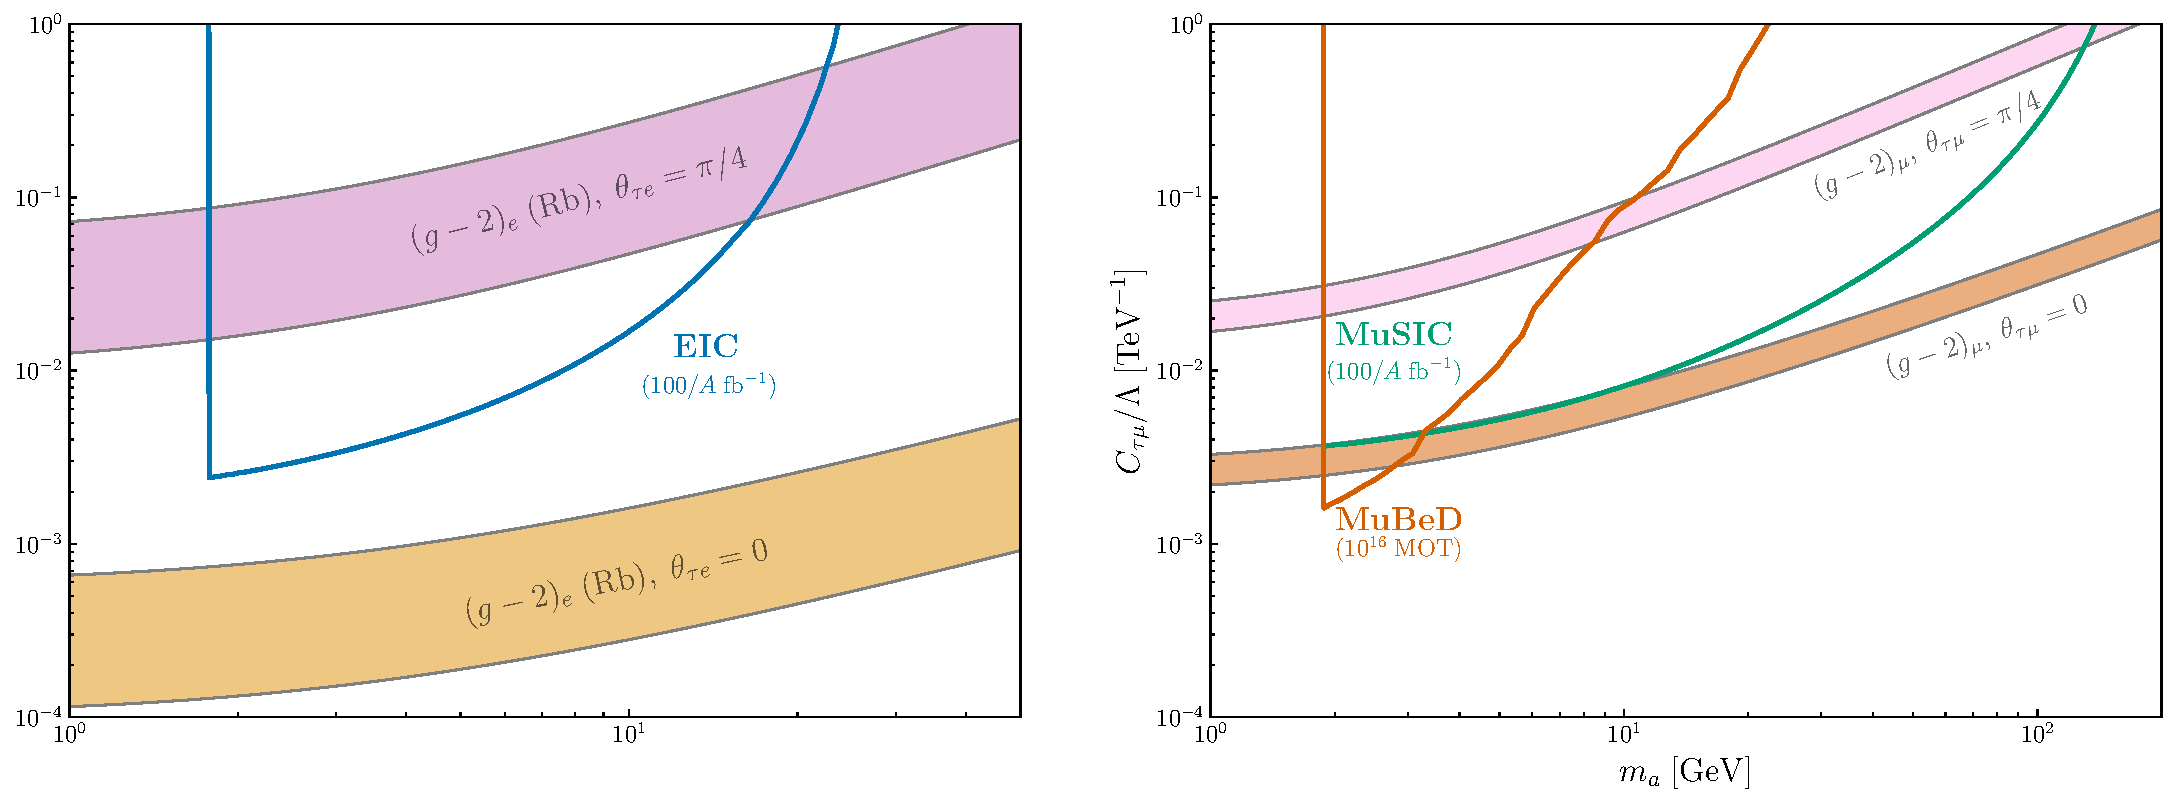
\includegraphics[width=\linewidth]{figures/chapter4/lfv_scalar_limits_and_g_2.pdf}
    \caption[Limits on LFV scalars at various lepton-nucleus collision experiments.]{(Left) limits on the $g_{\tau e}$ coupling at the EIC (assuming a $\tau$-identification efficiency of $\epsilon_\tau = 1\%$), alongside pure and chiral scalar explanations to the electron $g-2$ anomaly using $\alpha({\rm Rb})$. (Right) limits on the $g_{\tau \mu}$ coupling at MuSIC (assuming a $\tau$-identification efficiency of $\epsilon_\tau = 1\%$) and MuBeD (according to the analysis in the text), alongside pure and chiral scalar explanations to the muon $g-2$ anomaly.}
    \label{fig:scalar_limits}
\end{figure}
The only specific detector geometry we will consider is the pseudo-rapidity range. For the EIC, we take $|\eta| < 3.5$, whereas for MuSIC, we take $|\eta| < 6$. The latter choice is in line with the anticipated pseudo-rapidity reach of the B0 spectrometer at the EIC \cite{Adkins:2022jfp}. Given the additional beam energy and larger mass of the initial-state muon, we believe this is a reasonable detector requirement to ensure the final-state muon is able to be IDed.

For the muon fixed-target experiment MuBeD, we consider a set-up where the $1~{\rm TeV}$ muon beam is incident on a $2~{\rm cm}$ block of lead, instrumented on either end by veto and tracking layers, and accompanied on the far end by a spectrometer. We assume a modest number of muons on target, $N_{\mu} = 10^{16}$, which should be achievable in at most a few days of operation. For the signal, we require identification of the $\mu^+$ and both final state $\tau^-$. We expect that the experiment can be instrumented such that all 3-prong-decaying $\tau^-$ which have a decay length greater than $2~{\rm cm}$ can be identified. Given the boost of the final-state $\tau^-$ at such an experiment (see Fig.~\ref{fig:eta_gamma_fs_lepton}), this corresponds to a significant fraction of all $\tau^-$ produced in the interaction. Provided the charge of the leptons can be resolved, the identification of a $\mu^+\tau^-\tau^-$ final-state is a clear LFV signal with no SM background. 
\begin{figure}[t!]
    \centering
    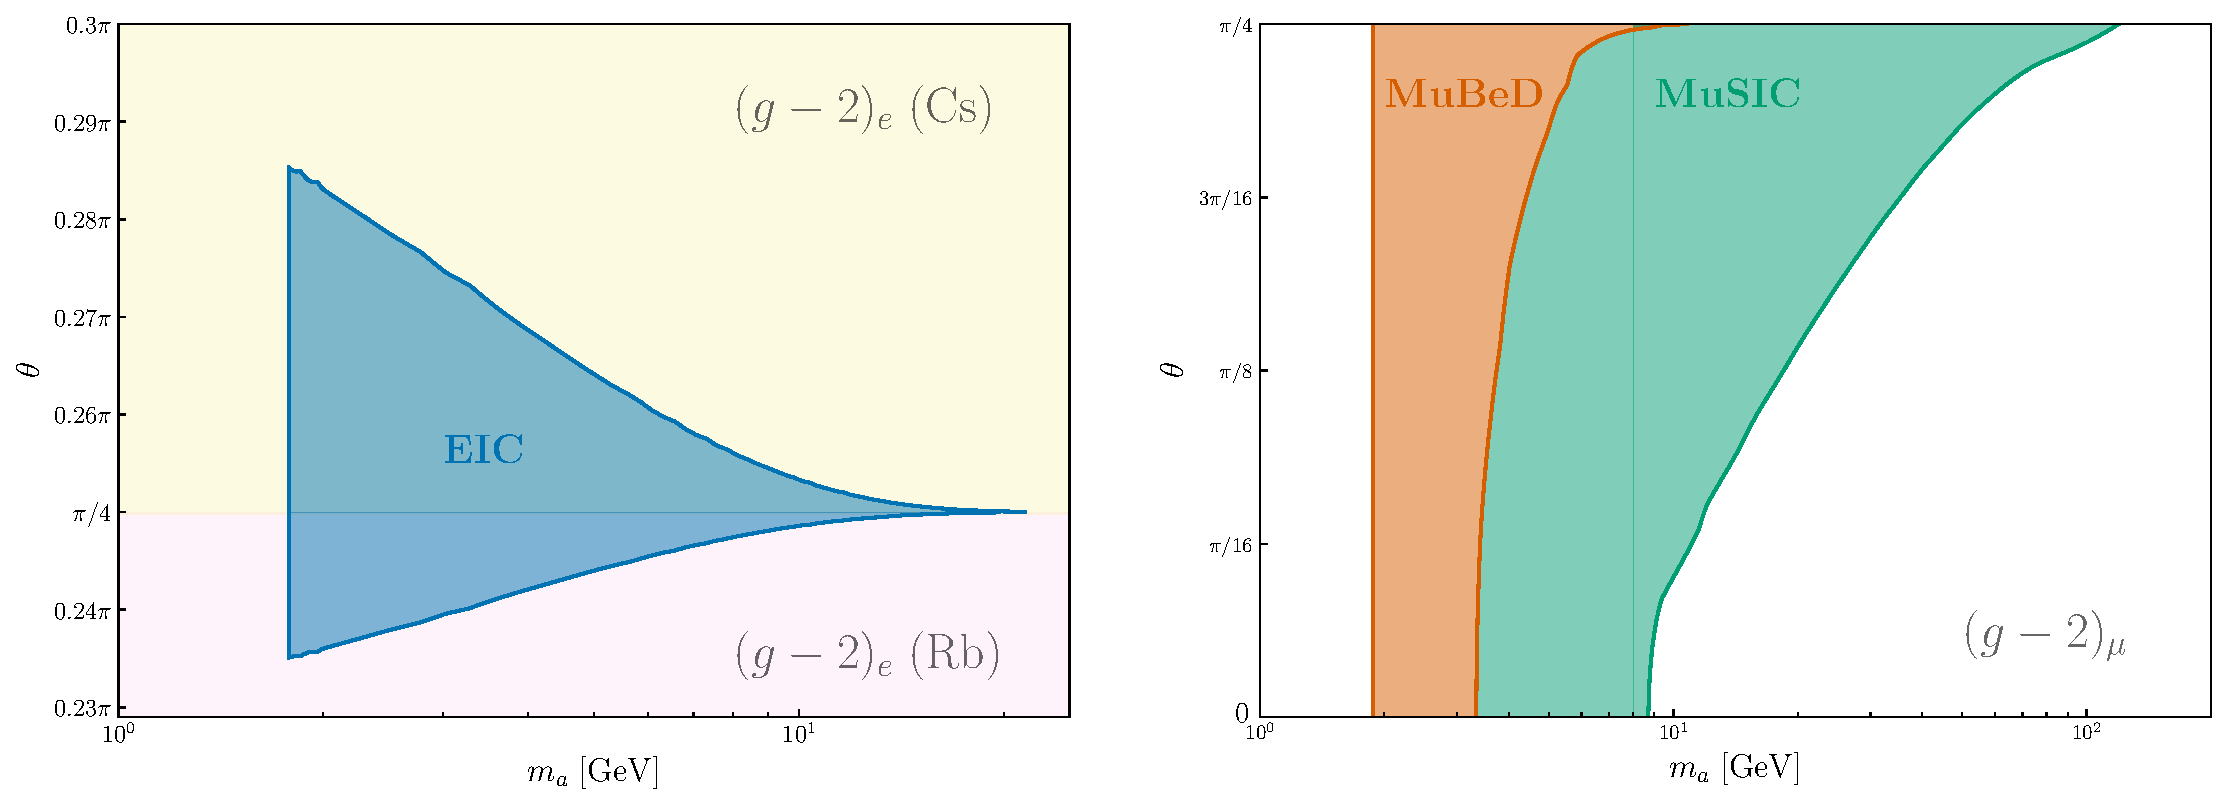
\includegraphics[width=\linewidth]{figures/chapter4/scalar_g_2_experiment_probes.pdf}
    \caption[Region in the $(m_\varphi, \theta_{\ell\tau})$ parameter space for which an LFV scalar $g-2$ explanation is probed within $2\sigma$ at various lepton-nucleus collision experiments.]{Region in the $(m_\varphi, \theta_{\ell\tau})$ parameter space for which a $g-2$ explanation is probed within $2\sigma$ at each of the colliders. In particular, the EIC is sensitive to explanations for {\it both} the Cesium and Rubidium electron $g-2$ anomalies depending on whether the angle $\theta_{e\tau}$ is above or below $\pi/4$. However, explanations to the muon $g-2$ anomaly require $\theta_{\mu\tau} < \pi/4$. The EIC is sensitive to chiral and near-chiral explanations of the electron $g-2$ anomalies, whereas both MuSIC and MuBeD probe nearly all explanations of the muon $g-2$ anomaly for GeV-scale $\varphi$.}
    \label{fig:scalar_explanations}
\end{figure}

We plot the results of the analyses in Fig.~\ref{fig:scalar_limits}. Interestingly, the parameter-space probed is very close to the LFV explanations to the electron and muon $g-2$ anomalies reviewed in Section \ref{sec:g-2_explanation}. To emphasize this point, we plot pure and chiral explanations to these anomalies alongside the limits. It appears that the EIC is able to probe chiral and near-chiral explanations of the electron $g-2$ anomaly (at least using $\alpha({\rm Rb})$, and MuBeD and MuSIC both explore nearly the entire parameter space of such explanations for GeV-scale $\varphi$. To get a better sense of the sensitivity of each experiment to these explanations, we plot the region of accessible solutions to the anomalies in the $(m_\varphi, \theta_{\tau\ell})$ plane in Fig.~\ref{fig:scalar_explanations}. 

In the event that the electron and muon anomalies are resolved, the ``explanations'' in Fig.~\ref{fig:scalar_limits} correspond roughly to constraints that one obtains from the magnetic dipole moment measurements, as shown in Fig.~\ref{fig:mdm_limits}. Then, we see that these experiments provide competitive and sometimes superior constraints, depending on the PV nature of the scalar interaction. Notably, while the limits from these experiments are nearly independent of the degree of PV angle for heavy $\varphi$, the limits from the magnetic dipole moment weaken considerably. However, it should be noted that such limits are superseded by limits from LFV lepton decays provided that additional couplings are non-zero, as is evident in Fig.~\ref{fig:LFV_limits}. Hence, while these experiments provide limits on the flavor-violating $g_{\ell\tau}$ coupling which are model-dependent up to the branching of the $\varphi$, the resulting limits are less sensitive than those obtained for models with generic non-zero couplings.
